%%%%%%%%%%%%%%%%%%%%%%%%%%%%%%%%%%%%%%%%
% Classe do documento
%%%%%%%%%%%%%%%%%%%%%%%%%%%%%%%%%%%%%%%%

% Nós usamos a classe "unb-cic".  Deixe apenas uma das linhas
% abaixo não-comentada, dependendo se você for do bacharelado ou
% da licenciatura.

\documentclass[bacharelado]{unb-cic}
%\documentclass[licenciatura]{unb-cic}



%%%%%%%%%%%%%%%%%%%%%%%%%%%%%%%%%%%%%%%%
% Pacotes importados
%%%%%%%%%%%%%%%%%%%%%%%%%%%%%%%%%%%%%%%%

\usepackage[brazil,american]{babel}
\usepackage[T1]{fontenc}
\usepackage{indentfirst}
\usepackage{natbib}
\usepackage[table,xcdraw]{xcolor}
\usepackage{color,soul}
\usepackage[utf8]{inputenc}
\usepackage{caption}
\usepackage{subfig}
\usepackage{graphicx}
\usepackage{multirow}
\usepackage{geometry}
\usepackage{listings}
\usepackage{pdfpages}

\usepackage{tikz}

\usetikzlibrary{arrows, calc, decorations.markings, positioning}
\setcounter{secnumdepth}{4}
\graphicspath{{./figuras/}}

% Para pular linha em células de tabela
\newcommand{\specialcell}[2][l]{%
  \begin{tabular}[#1]{@{}l@{}}#2\end{tabular}}

\pagestyle{empty}
\makeatletter
\newenvironment{timeline}[6]{%
    \newcommand{\startyear}{#1}
    \newcommand{\tlendyear}{#2}

    \newcommand{\yearcolumnwidth}{#3}
    \newcommand{\rulecolumnwidth}{#4}
    \newcommand{\entrycolumnwidth}{#5}
    \newcommand{\timelineheight}{#6}

    \newcommand{\templength}{}
    \newcommand{\entrycounter}{0}

    \long\def\ifnodedefined##1##2##3{%
        \@ifundefined{pgf@sh@ns@##1}{##3}{##2}%
    }
    \newcommand{\ifnodeundefined}[2]{%
        \ifnodedefined{##1}{}{##2}
    }

    \newcommand{\drawtimeline}{%
        \draw[timelinerule] (\yearcolumnwidth+5pt, 0pt) -- (\yearcolumnwidth+5pt, -\timelineheight);
        \draw (\yearcolumnwidth+0pt, -10pt) -- (\yearcolumnwidth+10pt, -10pt);
        \draw (\yearcolumnwidth+0pt, -\timelineheight+15pt) -- (\yearcolumnwidth+10pt, -\timelineheight+15pt);

        \pgfmathsetlengthmacro{\templength}{neg(add(multiply(subtract(\startyear, \startyear), divide(subtract(\timelineheight, 25), subtract(\tlendyear, \startyear))), 10))}
        \node[year] (year-\startyear) at (\yearcolumnwidth, \templength) {\startyear};
        \pgfmathsetlengthmacro{\templength}{neg(add(multiply(subtract(\tlendyear, \startyear), divide(subtract(\timelineheight, 25), subtract(\tlendyear, \startyear))), 10))}
        \node[year] (year-\tlendyear) at (\yearcolumnwidth, \templength) {\tlendyear};
    }

    \newcommand{\entry}[2]{
        \pgfmathtruncatemacro{\lastentrycount}{\entrycounter}
        \pgfmathtruncatemacro{\entrycounter}{\entrycounter + 1}

        \ifdim \lastentrycount pt > 0 pt%
            \node[entry] (entry-\entrycounter) [below of=entry-\lastentrycount] {##2};
        \else%
            \pgfmathsetlengthmacro{\templength}{neg(add(multiply(subtract(\startyear, \startyear), divide(subtract(\timelineheight, 25), subtract(\tlendyear, \startyear))), 10))}
            \node[entry] (entry-\entrycounter) at (\yearcolumnwidth+\rulecolumnwidth+10pt, \templength) {##2};
        \fi

        \ifnodeundefined{year-##1}{%
            \pgfmathsetlengthmacro{\templength}{neg(add(multiply(subtract(##1, \startyear), divide(subtract(\timelineheight, 25), subtract(\tlendyear, \startyear))), 10))}
            \draw (\yearcolumnwidth+2.5pt, \templength) -- (\yearcolumnwidth+7.5pt, \templength);
            \node[year] (year-##1) at (\yearcolumnwidth, \templength) {##1};
        }

        \draw ($(year-##1.east)+(2.5pt, 0pt)$) -- ($(year-##1.east)+(7.5pt, 0pt)$) -- ($(entry-\entrycounter.west)-(5pt,0)$) -- (entry-\entrycounter.west);
    }

    \newcommand{\plainentry}[2]{% plainentry won't print date in the timeline
        % #1 is the year
        % #2 is the entry text

        \pgfmathtruncatemacro{\lastentrycount}{\entrycounter}
        \pgfmathtruncatemacro{\entrycounter}{\entrycounter + 1}
        \ifdim \lastentrycount pt > 0 pt%
            \node[entry] (entry-\entrycounter) [below of=entry-\lastentrycount] {##2};
        \else%
            \pgfmathsetlengthmacro{\templength}{neg(add(multiply(subtract(\startyear, \startyear), divide(subtract(\timelineheight, 25), subtract(\tlendyear, \startyear))), 10))}
            \node[entry] (entry-\entrycounter) at (\yearcolumnwidth+\rulecolumnwidth+10pt, \templength) {##2};
        \fi

        \ifnodeundefined{invisible-year-##1}{%
            \pgfmathsetlengthmacro{\templength}{neg(add(multiply(subtract(##1, \startyear), divide(subtract(\timelineheight, 25), subtract(\tlendyear, \startyear))), 10))}
            \draw (\yearcolumnwidth+2.5pt, \templength) -- (\yearcolumnwidth+7.5pt, \templength);
            \node[year] (invisible-year-##1) at (\yearcolumnwidth, \templength) {};
        }

        \draw ($(invisible-year-##1.east)+(2.5pt, 0pt)$) -- ($(invisible-year-##1.east)+(7.5pt, 0pt)$) -- ($(entry-\entrycounter.west)-(5pt,0)$) -- (entry-\entrycounter.west);
    }

    \begin{tikzpicture}
        \tikzstyle{entry} = [%
            align=left,%
            text width=\entrycolumnwidth,%
            node distance=10mm,%
            anchor=west]
        \tikzstyle{year} = [anchor=east]
        \tikzstyle{timelinerule} = [%
            draw,%
            decoration={markings, mark=at position 1 with {\arrow[scale=1.5]{latex'}}},%
            postaction={decorate},%
            shorten >=0.4pt]

        \drawtimeline
}
{
    \end{tikzpicture}
    \let\startyear\@undefined
    \let\tlendyear\@undefined
    \let\yearcolumnwidth\@undefined
    \let\rulecolumnwidth\@undefined
    \let\entrycolumnwidth\@undefined
    \let\timelineheight\@undefined
    \let\entrycounter\@undefined
    \let\ifnodedefined\@undefined
    \let\ifnodeundefined\@undefined
    \let\drawtimeline\@undefined
    \let\entry\@undefined
}



%%%%%%%%%%%%%%%%%%%%%%%%%%%%%%%%%%%%%%%%
% Cores dos links
%%%%%%%%%%%%%%%%%%%%%%%%%%%%%%%%%%%%%%%%

% Veja o arquivos cores.tex se quiser ver que outras cores estão
% pré-definidas.  Utilizando o comando \hypersetup abaixo nós
% evitamos aquelas caixas vermelhas feias em volta dos links.

%%%%%%%%%%%%%%%%%%%%%%%%%%%%%%%%%%%%%%%%
% Cores do estilo Tango
%%%%%%%%%%%%%%%%%%%%%%%%%%%%%%%%%%%%%%%%

\definecolor{LightButter}{rgb}{0.98,0.91,0.31}
\definecolor{LightOrange}{rgb}{0.98,0.68,0.24}
\definecolor{LightChocolate}{rgb}{0.91,0.72,0.43}
\definecolor{LightChameleon}{rgb}{0.54,0.88,0.20}
\definecolor{LightSkyBlue}{rgb}{0.45,0.62,0.81}
\definecolor{LightPlum}{rgb}{0.68,0.50,0.66}
\definecolor{LightScarletRed}{rgb}{0.93,0.16,0.16}
\definecolor{Butter}{rgb}{0.93,0.86,0.25}
\definecolor{Orange}{rgb}{0.96,0.47,0.00}
\definecolor{Chocolate}{rgb}{0.75,0.49,0.07}
\definecolor{Chameleon}{rgb}{0.45,0.82,0.09}
\definecolor{SkyBlue}{rgb}{0.20,0.39,0.64}
\definecolor{Plum}{rgb}{0.46,0.31,0.48}
\definecolor{ScarletRed}{rgb}{0.80,0.00,0.00}
\definecolor{DarkButter}{rgb}{0.77,0.62,0.00}
\definecolor{DarkOrange}{rgb}{0.80,0.36,0.00}
\definecolor{DarkChocolate}{rgb}{0.56,0.35,0.01}
\definecolor{DarkChameleon}{rgb}{0.30,0.60,0.02}
\definecolor{DarkSkyBlue}{rgb}{0.12,0.29,0.53}
\definecolor{DarkPlum}{rgb}{0.36,0.21,0.40}
\definecolor{DarkScarletRed}{rgb}{0.64,0.00,0.00}
\definecolor{Aluminium1}{rgb}{0.93,0.93,0.92}
\definecolor{Aluminium2}{rgb}{0.82,0.84,0.81}
\definecolor{Aluminium3}{rgb}{0.73,0.74,0.71}
\definecolor{Aluminium4}{rgb}{0.53,0.54,0.52}
\definecolor{Aluminium5}{rgb}{0.33,0.34,0.32}
\definecolor{Aluminium6}{rgb}{0.18,0.20,0.21}

\hypersetup{
  colorlinks=true,
  linkcolor=DarkScarletRed,
  citecolor=DarkScarletRed,
  filecolor=DarkScarletRed,
  urlcolor= DarkScarletRed
}



%%%%%%%%%%%%%%%%%%%%%%%%%%%%%%%%%%%%%%%%
% Informações sobre a monografia
%%%%%%%%%%%%%%%%%%%%%%%%%%%%%%%%%%%%%%%%

\title{Avaliação de Interação Humano-Computador: um estudo de caso para bioinformática}

\orientador[a]{\prof \dr[a] Maria Emília Machado Telles Walter}{CIC/UnB}
%\coorientador[a]{\prof[a] \dr[a] Coorientadora}{MAT/UnB}
\coordenador{\prof \dr Rodrigo Bonifácio de Almeida}{CIC/UnB}
\diamesano{08}{Julho}{2016}

\membrobanca{\prof \dr[a] Fernanda Lima}{CIC/UnB}
\membrobanca{\prof \dr Professor II}{CIC/UnB}

\autor{Gabriella de Oliveira}{Esteves}
\CDU{004.4}

\palavraschave{Bioinformática, Redes Metabólicas, NoSQL, Grafo, Interação Humano-Computador, Método de Análise de Computabilidade}
\keywords{Bioinformatics, Metabolic Networks, NoSQL, Graph, Human-Computer Interaction,  Method for Evaluating Software Communicability}



%%%%%%%%%%%%%%%%%%%%%%%%%%%%%%%%%%%%%%%%
% Texto
%%%%%%%%%%%%%%%%%%%%%%%%%%%%%%%%%%%%%%%%

\begin{document}
  \maketitle
  \pretextual

  \begin{dedicatoria}
  Dedicatória
  \end{dedicatoria}

  \begin{agradecimentos}
  Agradecimento
  \end{agradecimentos}

  \begin{resumo}
  Resumo em português
  \end{resumo}

  \selectlanguage{american}
  \begin{abstract}
  Abstract in english
  \end{abstract}
  \selectlanguage{brazil}

  \tableofcontents
  \listoffigures
  \listoftables

  \textual 
  \chapter{Introdução}

% Dogma central

\indent No início dos anos 50, uma química britânica chamada Rosalind Frankling usou a técnica de difração de raios-X para determinação da estrutura da biomolécula do DNA e concluiu que sua forma era helicoidal. Seu trabalho foi empregado nos experimentos de dois pesquisadores, Francis Crick e James Watson, em um laboratório em Cambridge, e assim fizeram a grande descoberta que desencadearam várias linhas de pesquisas atuais: A partir do DNA, o processo de \textit{transcrição} fornece uma fita de RNA, que por sua vez, a partir do processo de \textit{tradução}, fornecem a proteína. Esta sequência de processos ficou conhecida como Dogma Central da biologia molecular.

% Atualmente

\indent A partir de então, pesquisadores já sequenciaram cadeias de DNA, RNA e proteína de vários organismos, criando uma quantidade de informação tão extensa que apenas ferramentas de Big Data podem ser usadas para análise, visualização, busca, etc, para um tratamento eficiente. Estes dados, denominados dados ômicos, são armazenados em bancos de dados específicos hoje em dia, mais vários deles colaboram entre si. Neste trabalho serão apresentados os bancos de dados que representam redes metabólicas em modelo de grafo já existentes, bem como suas ferramentas de visualização de vias metabólicas, e apresentar a ferramenta de visualização 2Path formularizada e desenvolvida neste projeto seguindo os padrões de projeto de interface do campo de Interface Humano-Computador. Para verificar se o sistema satisfaz os critérios básicos de qualidades (usabilidade, experiência de usuário, acessibilidade e comunicabilidade), este projeto utiliza um método de Interação Humano-Computador, chamado Método de Avaliação de Comunicabilidade, que fornece uma sequência de atividades a serem aplicadas para um grupo de pesquisadores biólogos e, ao final, coleta dados relativos à reação dos mesmos ao navegar no sistema.

% O que é metabolismo

% Quais moléculas fazem parte do metabolismo

% Como o metabolismo tem sido representado computacionalmente (redes metabólicas)

% Como as redes metabólicas tem sido visualizadas? (estado da arte)

\section{Justificativa}
\indent Atualmente, a quantidade de dados ômicos estudados pelos pesquisadores é extensa e complexa. Uma maneira de amenizar o esforço feito para analisá-los e compreendê-los é oferecer uma ferramenta que aproxime o usuário (pesquisador) e os dados e a maneira mais natural é representar tais dados em forma de grafo (redes metabólicas). Esta ferramenta deverá permitir que o usuário visualize e interaja com os dados dinamicamente.

\section{Problema}
\indent Construir uma visualização interativa,pelos padrões de interface sugeridos pela área de Interface Humano-Computador, de redes metabólicas armazenadas em banco de dados de grafos que permita ao pesquisador explorar os aspectos biológicos do organismo estudado.

\section{Objetivo}
\indent Construir um sistema que acesse redes metabólicas armazenadas em bancos de dados em grafo e gere uma visualização interativa e verificar se o sistema satisfaz os critérios de qualidade segundo o campo de Interação Humano-Computador.
\begin{itemize}
 \item Implementar uma busca das vias metabólicas de interesse a a partir de parâmetros informados pelo pesquisador no sistema;
 \item Recuperar a informação desejada e exibi-la para o pesquisador de forma ergonômica;
 \item Aplicar o Método de Avaliação de Computabilidade no sistema para medir a qualidade do mesmo.
\end{itemize}

\section{Descrição dos Capítulos}
\indent No Capítulo 1 serão apresentados os conceitos básicos de Interação Humano-Computador, métodos de avaliação da qualidade de sistemas computacionais com foco no Método de Avaliação de Comunicabilidade utilizado neste trabalho.
\indent No Capítulo 2 serão descritos os conceitos básicos de biologia molecular, metabolismo primário e secundário e os bancos de dados mais utilizados para armazenar as informações referentes às redes metabólicas. Também serão apresentados detalhadamente quatro ferramentas de visualização de redes metabólicas: \textit{Reactome Browser}, \textit{KEGG Pathway}, \textit{MetaCyc}, e \textit{2Path}. \\ 
\indent Os Capítulos 3 e 4 já são relacionados apenas ao sistema 2Path desenvolvido neste projeto. Enquanto o Capítulo 3 aborda o método de elaboração da interface auto-explicativa e consistente do sistema desde sua concepção incluindo certos detalhes sobre a implementação, o Capítulo 4 apresenta os resultados da aplicação do Método de Avaliação de Comunicabilidade definido no Capítulo 2 sobre o 2Path. \\
\indent O Capítulo 5  conclui o projeto e oferece sugestões para trabalhos futuros e, por fim, o Capítulo 6 descreve as atividades realizadas neste trabalho através de um cronograma. 
  \chapter{Biologia Molecular e Bioinformática}
 
\indent Neste capítulo serão descritos os conceitos básicos da biologia molecular. A seção \ref{aceidosNucleicos} define tais estruras e diferencia DNA de RNA por suas configurações e funções. A seção \ref{sinteseDeProteina} define as proteínas, apresenta seus quatro tipos diferentes e descreve o processo de sintetização de proteína. Por fim, a seção \ref{bioinformatica} estabelece os conceitos básicos dessa área, além de apontar os problemas atuais enfrentados nela. \\





%% ================================================================================================================== %%


\section{Ácidos Nucléicos} \label{aceidosNucleicos}

\indent Os ácidos nucléicos são biomoléculas responsáveis pelo armazenamento, transmissão e tradução das informações genéticas dos seres vivos. Isto é possível devido ao processo de síntede de proteínas que permite, assim, a base da herança biológica.Os acidos nucléicos são polímero, macromoléculas formadas por estruturas menores chamadas monômeros, que nesse caso são nucleotídeos. Nucleotídeos são compostos de três elementos: um radical fosfato (HPO$_{4}$), uma pentose, ou seja, um monossacarídeo formado por cinco átomos de carbono, e uma base nitrogenada. Existem cinco tipos de bases nitrogenadas que podem compor um nucleotídeo: Adenina(A), Timina(T), Citosina(C), Guanina(G) e Uracila(U). \\

\begin{figure}[h]
    \centering
    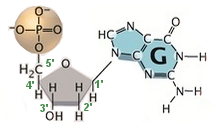
\includegraphics[width=0.5\textwidth]{nucleotideo.png}
    \caption{imagem de um nucleotídeo e das bases nitrogenadas. Mostrar backbone da pentose 1'...5'. Adaptado de : \cite{dnadiscovery08}. }
    \label{fig:Nucleotideo}
\end{figure} 

\indent Na figura \ref{fig:Nucleotideo}, observa-se que no \textit{backbone} do nucleotídeo existe uma numeração de 1' à 5', que representam os carbonos presentes na pentose. Para a criação de uma fita de ácido nucléico, no processo de polimerização fomar-se uma ligação fosfodiéster entre o carbono da posição 5' do \textit{backbone} de um nucleotídeos e o carbono de posição 3' do \textit{backbone} de outro \cite{setubal97}. Por definição o sentido da leitura de uma fita de ácido nucléido é 5' $\rightarrow$ 3', o que é deve ser levado em consideração ao se fazer interpretação de dados do material genético. \\

\indent Dois tipos de ácidos nucléicos são encontrados nos seres vivos: ácido desoxirribonucleico (DNA) e ácido ribonucleico (RNA). Eles diferenciam-se tanto na estrutura do \textit{backbone} e nas bases nitrogenadas, quanto em suas funções. A seguir serão apresentadas as definições de DNA e RNA.

\subsection{DNA} \label{aceidosNucleicos:dna}

\indent Os DNAs (ou ADN - Ácido Desoxirribonucleico) são as biomoléculas que armazenam as informações referentes ao funcionamento de todas as células dos seres vivos de maneira específica: sequências de pares de bases nitrogenadas. Nesse sentido, além de haver a ligação fosfodiéster entre os nucleotídeos, cada um também se liga a partir de suas bases nitrogenadas, formando assim um eixo helicoidal tridimensional chamada de dupla hélice \cite{setubal97}. Esta estrutura foi descoberta em 1953, pelo biólogo James Watson e pelo físico Francis Crick \cite{dnadiscovery08}, porém os ácidos nucléicos já eram estudado desde 1869 na Suíça pelo químico-fisiológico Friedrich Miescher. \\

\indent Em relação à estrutura dos monômeros do DNA, o \textit{backbone} dos nucleotídeos é uma desoxirribose, indicada na figura \ref{fig:EstruturasDoDNA}. Para a formação da dupla hélice, os pares são feitos com uma base nitrogenada do grupo de purinas, composto orgânico que possui um anel duplo de carbono, e outra base do grupo de pirimidinas, composto orgânico que possui um anel simples de carbono. No caso do DNA, somente quatro das cinco bases são empregadas: as purinas Adenina(A) e Guanina(G), que se ligam com as pirimidinas Timina(T) e Citosina(C) respectivamente. Desta forma, A e T são bases complementares, assim como G e C. Uma fita de DNA pode conter centenas de milhões de nucleotídeos. \\

\indent A representação do DNA, seja nos livros ou computacionalmente, é dada por um par em paralelo de strings de letras A, T, G e C. Como explicado no início dessa seção, o sentido padrão da leitura de uma fita é de 5' $\rightarrow$ 3', mas no caso do DNA, as hélices são dispostas de maneira antiparalela, ou seja, uma é lida de 5' $\rightarrow$ 3' e a outra, de 3' $\rightarrow$ 5'. Observa-se que a partir de uma hélice, pode-se inferir a sequência de sua hélice complementar. Seja, por exemplo, uma hélice H1 igual a AGTAAGC; então H2 em seu sentido oposto é H2' igual a TCATTCG, e no sentido regular, igual a GCTTACT. A figura \ref{fig:EstruturasDoDNA} apresenta a estrutura do DNA como explicada nesta seção. \\

\begin{figure}[h]
    \centering
    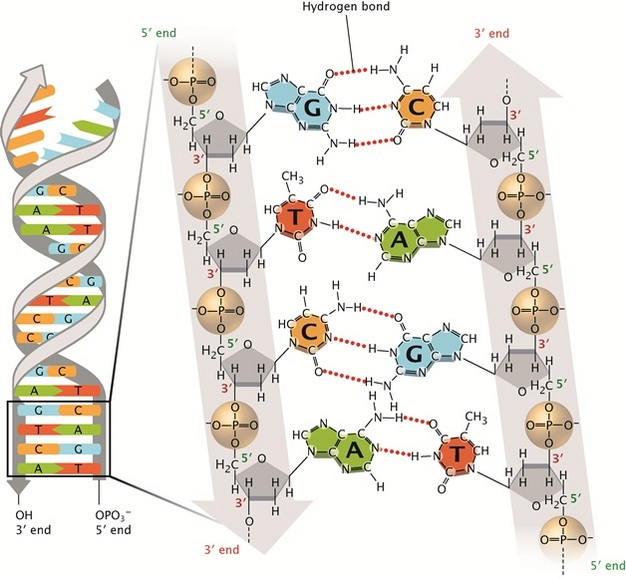
\includegraphics[width=0.7\textwidth]{dnaEstrutura.jpg}
    \caption{Adaptado de : \cite{dnadiscovery08} }
    \label{fig:EstruturasDoDNA}
\end{figure} 


\subsection{RNA} \label{aceidosNucleicos:rna}

\indent Os RNAs são biomoléculas semelhantes ao DNA, porém contam com três diferenças básicas. A primeira é a estrutura do \textit{backbone} dos nucleotídeos, que é composta por uma ribose ao invés de um desoxirribose. A segunda difereça é em relação às bases nitrogenadas, onde a pirimidina Uracila(U) substitui a Timita(T). 
Por fim, o RNA é formado por apenas uma hélice tridimensional. \\

\indent Existem três tipos de RNAs presentes no citoplasma - espaço entre a membrama plasmática e o núcleo da célula. 
Cada um possui funções específicas que serão detalhadas na seção \ref{transcricaoTraducaoSintese}. Em suma, O RNA mensageiro (mRNA) é responsável pela transferência de informação do DNA para o RNA ribossômico (rRNA), que por sua vez irá desanexar a proteína do RNA transportador (tRNA) combinando-o com o rRNA, executando assim, a síntese de proteína. \\



%% ================================================================================================================== %%

\section{Síntese de Proteína} \label{sinteseDeProteina}



\subsection{Proteína} \label{sinteseDeProteina:proteina}

\indent As proteínas são biomoléculas com diversas responsabilidades no corpo dos seres vivos. 
Se fizerem parte do no grupo de proteínas fibrosas, como o colágeno, irão compor a estrutura do corpo e para isso precisam ser resistentes e insolúveis em água. Caso estejam no grupo de proteínas globulares, como a hemoglobina, realizarão processos dinâmico pelo corpo tais como transportações e cataliações \cite{profangela11}.  Cada tarefa é realizada por um proteína com uma estrutura específica e otimizada pra tal. \\

\indent Assim como os ácidos nucléicos, as proteínas são polímeros, macromoléculas cujos monômeros são aminoácidos. Aminoácidos são moléculas que possuem cinco componentes: amina (NH$_{2}$), carbono (C), hidrogênio (H), ácido carboxílico (COOH) e uma cadeia lateral que funciona como identificador de cada um dos 20 tipos de aminoácidos presentes nos seres vivos. A maneira como eles são criados será explicada com mais detalhes na subseção \ref{sinteseDeProteina:transcricaoTraducaoSintese}, pois envolve um processo complexo de síntese de proteína executado pelo ribossomo. A ligação, ou polimerização, de dois aminoácidos é feita unindo a amida de um com o ácido carboxílico do outro, liberando uma molécula de água (H$_{2}$O) e formando uma cadeia chamada de dipeptídeo. Como houve liberação de água na ligação, o dipeptídeo não é formado por aminoácidos, mas sim resíduos dos mesmos. Nesse sentido, cadeias peptídicas de 100 à 5000 diferentes resíduos aminoácidos, ou cadeia polipeptídicas,  constituem a proteína. \\

\indent Existem quatro estruturas para caracterização de uma proteína \cite{setubal97}. A mais simples é chamada de estrutura primária e é composta por uma sequência linear de resíduos aminoácidos. A estrutura secundária é tridimensional e estabiliza-se por meio de ligações de hidrogênio na cadeia principal, chamada de \textit{backbone}. Dependendo da disposição dos resíduos de aminoácidos, esta cadeia pode se dar forma de hélice ou em forma de folha. A estrutura terciária é dada pela união de várias estruturas secundárias e, por fim, a estrutura quaternária é composta de múltiplas estruturas terciárias \cite{drug09}. A figura \ref{fig:EstruturasDaProteina} ilustra os quatro tipos de proteínas descritos. \\

\begin{figure}[h]
    \centering
    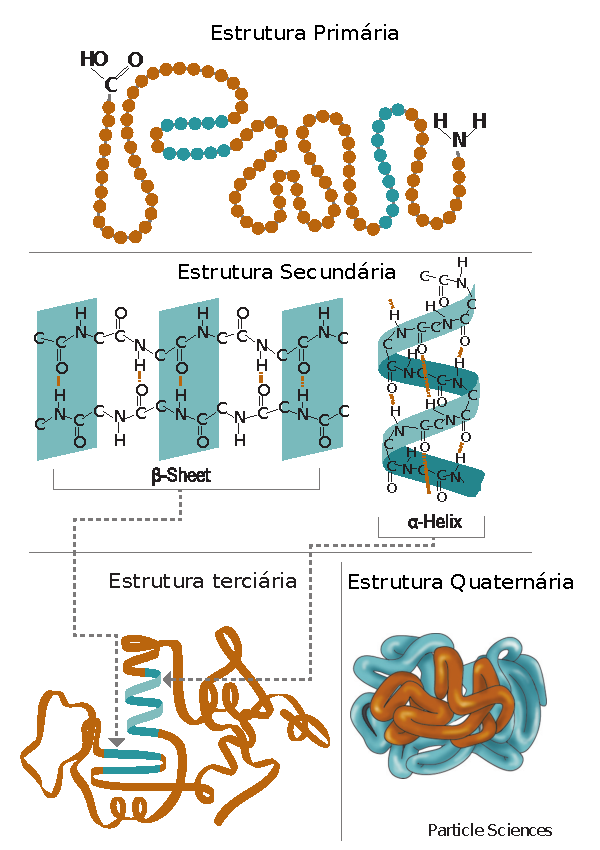
\includegraphics[width=0.6\textwidth]{EstruturasDaProteina.pdf}
    \caption{Adaptado de : \cite{drug09} }
    \label{fig:EstruturasDaProteina}
\end{figure}

\subsection{Código Genético} \label{sinteseDeProteina:codigoGenetico} 

\indent No núcleo de cada célula eucariota, ou no citoplasma das células procariotas, estão localizados as moléculas de DNA, chamadas individualmente por \textbf{cromossomo}. O número de cromossomos em cada célula varia por espécie. No caso dos chimpanzés, o núcleo das células possui 48 cromossomos e no caso dos seres humanos, 46. Note que não existe relação entre o grau evolutivo das espécies e o número de cromossomos nas células. \\ 

\indent Um cromossomo pode ser representado por vários trechos contíguos de DNA, sendo que cada trecho é chamado de \textbf{gene}, ou locus - local fixo no cromossomo. Portanto, pode-se afirmar que o cromossomo é um conjunto (ou lista) de genes. No caso dos seres humanos, o número de genes em cada célula gira em torno de 22 mil,
% Fonte: http://www.ncbi.nlm.nih.gov/pmc/articles/PMC2898077/
 e o genoma humano possui em média 3 bilhões de pares de bases. Poderíamo inferir, então, que a média de pares de bases por gene é de $\frac{3.000.000.000}{22.000} \simeq 136.000$, porém este cálculo é muito generalizado e equivocado, uma vez que os genes possuem tamanhos diferentes, onde o maior possui 250 milhões de pares, enquanto o menor possui apenas 50 milhões, no caso dos seres humanos. % Fonte: http://www.objetivo.br/noticias.asp?id=3692}
  Um gene, por sua vez, pode ser representado por vários trechos de três pares de base, sendo que cada trecho é chamado de \textbf{códon}. \\

\indent Normalmente cada proteína é formada a partir de um gene particular. Mais especificamente, cada aminoácido da proteína é formado a partir de um códon do gene. Entretanto, existem 64 códon possíveis ($4_{ParesDeBase} ^3$) mas somente 20 aminoácidos a serem codificados. Nesse sentido, é comum haver mais de um códon correspondendo à um aminoácio. Além disso, 3 destes códons são responsáveis por indicar o final de uma proteína. O mRNA é encarregado de transportar a informação da sequência correta para construção de proteína, em forma de sequência de códons. A tabela \ref{tabelaCodigoGenetico} que apresenta a correspondência entre códons e aminoácios é chamada de \textbf{código genético} \cite{setubal97}, e a tabela \ref{tabelaAminoacidos} apresenta o código genético codificado em letras do alfabeto utilizado atualmente para comparação entre proteínas. Note que as bases nitrogenadas são do RNA, e não do DNA, pois é a molécula do primeiro que faz a conexão entre DNA e a proteína, num processo que será explicado na próxima subseção. \textbf{BUSCAR FONTE DISSO} \\

\indent A partir destas tabelas, podemos montar o seguinte exemplo: Suponha que a palvra GENETICA seja uma proteína. Então existe uma configuração de aminoácidos que forma essa proteína, e ela pode ter a forma: \\ 
\indent GENETICA $\leftarrow$ Glicina - Glutamano - Metionina - Glutamano \\
\hspace*{3.4cm}  Treonina - Isoleucina - Cisteina - Alanina \\
\indent GENETICA $\leftarrow$ Gly - Glu - Asn - Glu - Thr - Ile - Cys - Ala \\
\indent GENETICA $\leftarrow$ GGG - GAG - AAC - GAA - ACG - AUC - UGC - UCC \\


\begin{table}[h!] 
\centering
%\captionsetup{labelsep=space,justification=justified,singlelinecheck=off}
\caption{Código Genético} \label{tabelaCodigoGenetico}
\begin{tabular}{|c|c|c|c|c|c|c|c|}
\hline
 \multirow{2}{*}{ \begin{tabular}[x]{@{}c@{}} Primeira \\ Posição \end{tabular} } & 
 \multicolumn{4}{|c|}{Segunda Posição} & 
 \multirow{2}{*}{ \begin{tabular}[x]{@{}c@{}} Terceira \\ Posição \end{tabular} }\\  \cline{2-5}
 & G & A & C & U &  \\ \hline
 
 \multirow{5}{*}{G} & Gly & Glu & Ala & Val & G \\ 
 					& Gly & Glu & Ala & Val & A \\ 
 					& & & & & 					 \\ 
 					& Gly & Asp & Ala & Val & C \\ 
 					& Gly & Asp & Ala & Val & U \\ \hline 
 					
 \multirow{5}{*}{A} & Arg & Lys & Thr & Met & G \\ 
 					& Arg & Lys & Thr & Ile & A \\ 
 					& & & & & 					 \\ 
 					& Ser & Asn & Thr & Ile & C \\ 
 					& Ser & Asn & Thr & Ile & U \\ \hline 
 					
 \multirow{5}{*}{C} & Arg & Gln & Pro & Leu & G \\ 
 					& Arg & Gln & Pro & Leu & A \\ 
 					& & & & & 					 \\ 
 					& Arg & His & Pro & Leu & C \\ 
 					& Arg & His & Pro & Leu & U \\ \hline 
 					
 \multirow{5}{*}{U} & Trp & \textbf{FIM} & Ser & Leu & G \\ 
 					& \textbf{FIM} & \textbf{FIM} & Ser & Leu & A \\ 
 					& & & & & 					 \\ 
 					& Cys & Tyr & Ala & Phe & C \\ 
 					& Cys & Tyr & Ala & Phe & U \\ \hline 
 
\end{tabular}
\end{table}




\begin{table}[h!] 
\centering
%\captionsetup{labelsep=space,justification=justified,singlelinecheck=off}
\caption{Aminoácidos codificados} \label{tabelaAminoacidos}
\begin{tabular}{|c|c|c|c|} \hline
& Aminoácido & Abreviação & Código no alfabeto  \\  \hline
1 & Alanina & Ala & A \\ 
2 & Cisteina & Cys & C \\ 
3 & Aspartano ou Ácido aspártico & Asp & D \\ 
4 & Glutamato ou Ácido glutâmico & Glu & E \\ 
5 & Fenilalanina & Phe & F \\ 
6 & Glicina ou Glicocola & Gly & G \\ 
7 & Histidina & His & H \\ 
8 & Isoleucina & Ile & I \\ 
9 & Lisina & Lys & K \\ 
10 & Leucina & Leu & L \\ 
11 & Metionina & Met & M \\ 
12 & Asparagina & Asn & N \\ 
13 & Prolina & Pro & P \\ 
14 & Glutamina & Gln & Q \\ 
15 & Arginina & Arg & R \\ 
16 & Serina & Ser & S \\ 
17 & Treonina & Thr & T \\ 
18 & Valina & Val & V \\ 
19 & Tripofano & Trp & W \\ 
20 & Tirosina & Tyr & Y \\ \hline
 
\end{tabular}
\end{table}



\subsection{Transcrição e tradução} \label{sinteseDeProteina:transcricaoTraducaoSintese}


%CÓPIA DO SETUBAL. MUDAR DEPOIS !!!!!!!!

%% -----------------------------------------------------------------
%% -----------------------------------------------------------------
%% -----------------------------------------------------------------

\indent Finalmente, agora será descrita a forma como as informações contidas no DNA resulta em proteínas. Um mecanismo de célula reconhece o início de um gene ou aglomerado de genes graças ao \textit{promotor}. O promotor é uma região antes de cada gene no DNA que serve como uma indicação para o mecanismo celular que é um gene está a frente. O códon AUG (que é codificado para metionina) também indica o início de um gene. Tendo reconhecido o início de um gene ou \textit{cluster} de genes, uma cópia do gene é feita sobre uma molécula de RNA. Este RNA resultante é o RNA mensageiro, ou mRNA, e terá exatamente a mesma sequência que uma das cadeias do gene, mas substituindo U por T. Este processo é chamado de \textbf{transcrição}. O mRNA, então, será utilizado em estruturas celulares chamados ribossomas para a fabricação de uma proteína. \\

\indent Uma vez que o RNA é de cadeia simples e DNA é de cadeia dupla, o mRNA produzido é idêntico em sequência à apenas uma das cadeias do gene, sendo complementar à outra cadeia - lembrando que T é substituído por U no RNA. A vertente que se parece com o produto mRNA é chamado de anti-sentido ou cadeia codificadora, e o outro é o sentido ou anticodificação ou cadeia de molde. A cadeia de molde é aquele que é transcrita, pois o mRNA é composto por ligações de ribonucleotidos complementares a esta vertente. O processo sempre contrói moléculas de mRNA da extremidade 5' até a 3', ao passo que a cadeia de molde é lida de 3' para 5 '. Note também que a cadeia de molde não é sempre a mesma; Por exemplo, a cadeia de molde para um determinado gene A pode ser uma das fitas, e a cadeia de molde para outro gene B pode ser a outra fita. Para um dado gene, a célula é capaz de reconhecer os correspondentes moldes de cadeia graças ao promotor. Mesmo que o complemento reverso do promotor aparece na outra cadeia, ele não é um promotor e por isso não irá ser reconhecido como tal. Uma consequência importante deste fato é que os genes do mesmo cromossomo tem uma orientação com relação ao outro: Dado dois genes, se eles aparecem na mesma vertente eles têm a mesma orientação; caso contrário, eles têm orientação oposta. Finalmente, note que os termos \textit{upstream} e \textit{downstream} são usados para indicar as posições do DNA em referência à orientação da cadeia codificadora, com o promotor sendo o \textit{upstream} do gene. \\

\indent A transcrição descrita é válida para os organismos classificados como procariontes. Estes organismos têm o seu DNA livre na célula, pois não há uma membrana nuclear. Exemplos de procariontes são bactérias e algas azuis. Todos os outros organismos, categorizados como eucariotas têm um núcleo separado do resto da célula por uma membrana nuclear, e o seu DNA é mantido no interior do núcleo. Nestes organismos a transcrição genética é mais complexa. Muitos genes eucarióticos são compostos por partes alternadas dos chamados \textit{introns} e \textit{exons}. Após a transcrição, os \textit{introns} são unidos fora do mRNA. Isto significa que os \textit{introns} são partes de um gene que não são utilizados na síntese de proteínas. Depois que os \textit{introns} são unidos, o mRNA encurtado (contendo cópias apenas dos \textit{exons} e de regiões reguladoras nas extremidades), deixa o núcleo, uma vez que os ribossomos estão fora. \\

\indent Devido ao fenômeno de \textit{introns/exons}, serão usados nomes diferentes para se referir ao gene como um todo encontrado no cromossomo e a sequência de \textit{splicing}, \textit{exons} unidos. O primeiro é chamado de DNA genômico e o segundo de DNA complementar ou DNAc. Os cientistas podem fabricar DNAc sem saber o seu homólogo genômico. Eles primeiro capturam o mRNA fora do núcleo no seu caminho para os ribossomos. Em seguida, num processo denominado \textbf{transcrição reversa}, que produzem moléculas de DNA utilizando o mRNA como um molde. Uma vez que o mRNA contém apenas os \textit{exons}, esta é também a composição do DNA produzido. Assim, eles podem obter cDNA sem sequer olhar para os cromossomos. Ambos transcrição e transcrição reversa são processos complexos que necessitam a ajuda de enzimas. Transcriptase e transcriptase reversa são os enzimas que catalisam a estes processos na célula. Há também um fenômeno chamado de \textit{splicing} alternativo. Isto ocorre quando o mesmo DNA genômico pode dar origem a duas ou mais moléculas de mRNA diferentes, escolhendo os \textit{introns} e \textit{exons} de maneiras diferentes. Eles em geral produzem proteínas diferentes. \\

\indent Voltando ao mRNA e síntese protéica, dois outros tipos de moléculas RNA desempenham papéis muito importantes. Como já mencionado, a síntese de proteína é realizada dentro de estruturas celulares chamadas ribossomos. Os ribossomas são feitos de proteínas e uma estrutura de RNA denominada RNA ribossômico, ou rRNA. Os ribossomos funcionam como uma linha de montagem em uma fábrica usando como \textit{inputs} uma molécula de mRNA e outro tipo de molécula de RNA chamado RNA de transferência, ou tRNA. \\

\indent tRNAs são as moléculas que realmente implementam o código genético em um processo chamado de \textbf{tradução}. Elas fazem a conexão entre um códon e o aminoácido específico este códons codifica. A medida que o mRNA passa através do interior do ribossomo, um tRNA correspondente ao códon corrente - o códon no mRNA atualmente no interior do ribossomo - se liga a ele, trazendo o aminoácido correspondente (vários aminoácidos livres estão sempre em torno da célula). A posição tridimensional de todas essas moléculas neste momento é tal que, assim que o tRNA se liga ao seu códon, o aminoácido ligado vai para o lado do aminoácido precedente na cadeia de proteína que está sendo formada. Uma enzima adequada catalisa então a adição deste aminoácido corrente para a cadeia de proteína, libertando-o do tRNA. Uma proteína é construída, resíduo por resíduo, desta forma. Quando um códon de parada aparece, nenhum tRNA é associado à ele e a síntese termina. O RNA mensageiro é liberado e degradados por mecanismos celulares em ribonucleotidos, que serão em seguida reciclados para fazer outros RNAs. \\


%% -----------------------------------------------------------------
%% -----------------------------------------------------------------
%% -----------------------------------------------------------------


\cite{setubal97}



%% -----------------------------------------------------------------
%% -----------------------------------------------------------------
%% -----------------------------------------------------------------



\begin{figure}[h]
    \centering
    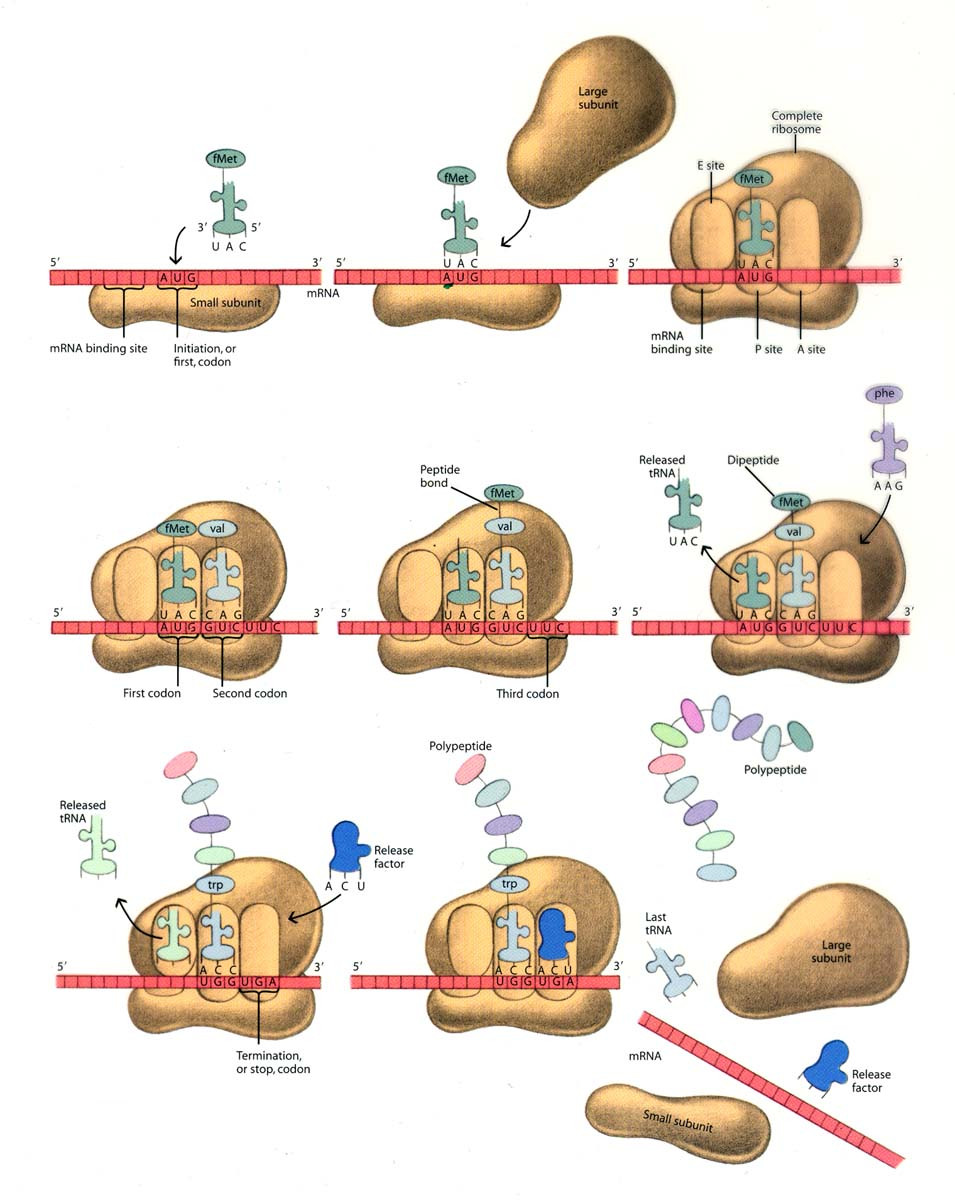
\includegraphics[width=0.9\textwidth]{transcricaoEtraducao.jpeg}
    \caption{Adaptado de : http://www.stepbystep.com/difference-between-transcription-and-translation-in-dna-103278/ }
    \label{fig:transcricaoEtraducao}
\end{figure}




\section{Bioinformática} \label{bioinformatica}

\subsection{Sequenciamento} 

\indent Mardis 2008

\subsection{Desafio das ômicas}

\indent 
Genômica

\indent Conceitualização do algortimo.

Artigos:
Introdução
[introduction to bioinformatics for computer scientists]


  \chapter{IHC}

%http://acervodigital.ufpr.br/bitstream/handle/1884/36666/Luiz%20Augusto%20Sakakibara.pdf?sequence=1
  \chapter{2Path}

% =========================================================================================

\section{Projeto de Interface}


\subsection{Tabela de Interações}

\indent 
\begin{table}
\centering
\caption{Representação da interação entre usuário (U) e projetista (P). Os signos representam o foco de cada conversa.} \label{tabelaDeInteracao:2Path}
\begin{tabular}{|l|l|}
\hline
{\cellcolor[HTML]{DFDFDF}\textbf{\specialcell{Tópico\\>Subtópico (diálogo)}}} &  {\cellcolor[HTML]{DFDFDF}\textbf{\specialcell{Falas e Signos\\U: Usuário e P: Projetista}}} \\ \hline 
Pesquisar enzima & \specialcell{\textbf{U}: Quero procurar uma \textit{enzima} no banco de dados 2Path.} \\ \hline
\specialcell{> Informar dados\\da enzima}	& \specialcell{\textbf{P}: Qual o \textbf{número EC} (\textit{Enzyme Commission})\\da enzima?} \\ 
				  & \specialcell{\textbf{U}: O número EC é (...).} \\ 
				  & \specialcell{\textbf{P}: OK. A enzima está no banco de dados e ela catalisa as\\\textbf{reações} (...) cujos \textbf{substratos} são (...) e os \textbf{produtos}\\são (...).} \\ \hline
\specialcell{Pesquisar enzima\\em organismo} & \specialcell{\textbf{U}: Quero saber se o genoma de um dos meus organismos\\possui sequencia que produz certa enzima.} \\ \hline
> Informar organismo & \specialcell{\textbf{P}: Em qual dos seus \textbf{organismos} você quer buscar essa\\enzima?} \\
& \specialcell{\textbf{U}: O organismo é (...).} \\ \hline
\specialcell{> Informar dados\\da enzima} & \specialcell{\textbf{P}: Qual o \textbf{número EC} da enzima?} \\
& \specialcell{\textbf{U}: O número EC é (...).} \\ 
& \specialcell{\textbf{P}: OK. A está no banco de dados e ela catalisa as\\\textbf{reações} (...) cujos \textbf{substratos} são (...) e os \textbf{produtos}\\são (...). O organismo (...) possui as sequências (...) que\\produziram tal enzima.} \\ \hline

\specialcell{Procurar caminho\\entre dois\\metabólitos} & \specialcell{\textbf{U}: Quero saber se um certo metabólito é substrato de\\alguma \textbf{via} \textbf{metabólica} no 2Path cujo produto é um\\outro certo metabólito.} \\ \hline
\specialcell{> Informar dados\\dos metabólitos} & \specialcell{\textbf{P}: Qual o \textbf{substrato}? Qual o \textbf{produto}?} \\
&  \specialcell{\textbf{U}: O substrato é (...) e o produto é (...).} \\
& \specialcell{\textbf{P}: OK. Existe uma via que liga estes dois metabólitos.\\As \textbf{reações} (...) e os \textbf{compostos} (...) estão entre eles.} \\ \hline
\specialcell{Procurar caminho\\entre dois\\metabólitos\\em organismo} & \specialcell{\textbf{U}: Agora quero verificar se há uma via metabólica entre\\dois metabólitos em um dos meus organismos.} \\ \hline
> Informar organismo & \specialcell{\textbf{P}: Em qual dos seus \textbf{organismos} você quer buscar essa\\enzima?} \\
& \specialcell{\textbf{U}: O organismo é (...).} \\ \hline
\specialcell{> Informar dados\\da metabólitos} & \specialcell{\textbf{P}: Qual o \textbf{substrato}? Qual o \textbf{produto}?} \\
&  \specialcell{\textbf{U}: O substrato é (...) e o produto é (...).} \\
& \specialcell{\textbf{P}: OK. Existe uma via que liga estes dois metabólitos.\\O \textbf{organismo} possui as \textbf{sequências} (...) que geram \\as \textbf{enzimas} (...) que, por sua vez, catalisam as \textbf{reações}.\\Estas são as reações que compõem a via metabólica\\e os \textbf{compostos} (...) são seus substratos e produtos.} \\ \hline

\end{tabular}
\end{table}

\subsection{Mapa de Objetivos}

\indent O 2Path foi desenvolvido considerando que um usuário já fez \textit{login} no sistema e já possui pelo menos um organismo em seu banco de dados particular. Nesse sentido, o usuário possui dois objetivos finais:
\begin{itemize}
\item[1]: Verificar se existe uma via metabólica entre dois compostos no banco de dados público do 2Path e/ou em algum de seus organismos privados;
\item[2]: Verificar se existe uma enzima específica no banco de dados público do 2Path e/ou em algum dos seus organismos privados. 
\end{itemize}

\indent Para atingir tais objetivos, ele precisa realizar certos objetivos instrumentais diretos e indiretos. Observe que a manipulação do grafo na visualização da via metabólica envolve clicar, mover e passar o mouse por cima nos nós e arestas.
\begin{itemize}
\item[Direto]: Informar dois elementos: substrato e produto;
\item[Direto]: Informar enzima;
\item[Direto]: Manipular grafo para obter informações sobre os nós e arestas;
\item[Indireto]: Fazer \textit{login} no sistema (Considerado já feito);
\item[Indireto]: Fazer \textit{upload} de arquivos FASTA de organismos (Considerado já feito).
\end{itemize}

\indent A Figura \ref{fig:mapaDeObjetivos} apresenta o Mapa de Objetivos do sistema 2Path construído com base nos objetivos finais e instrumentais (diretos e indiretos) dos usuários. 

\begin{figure}[!h]
    \centering
    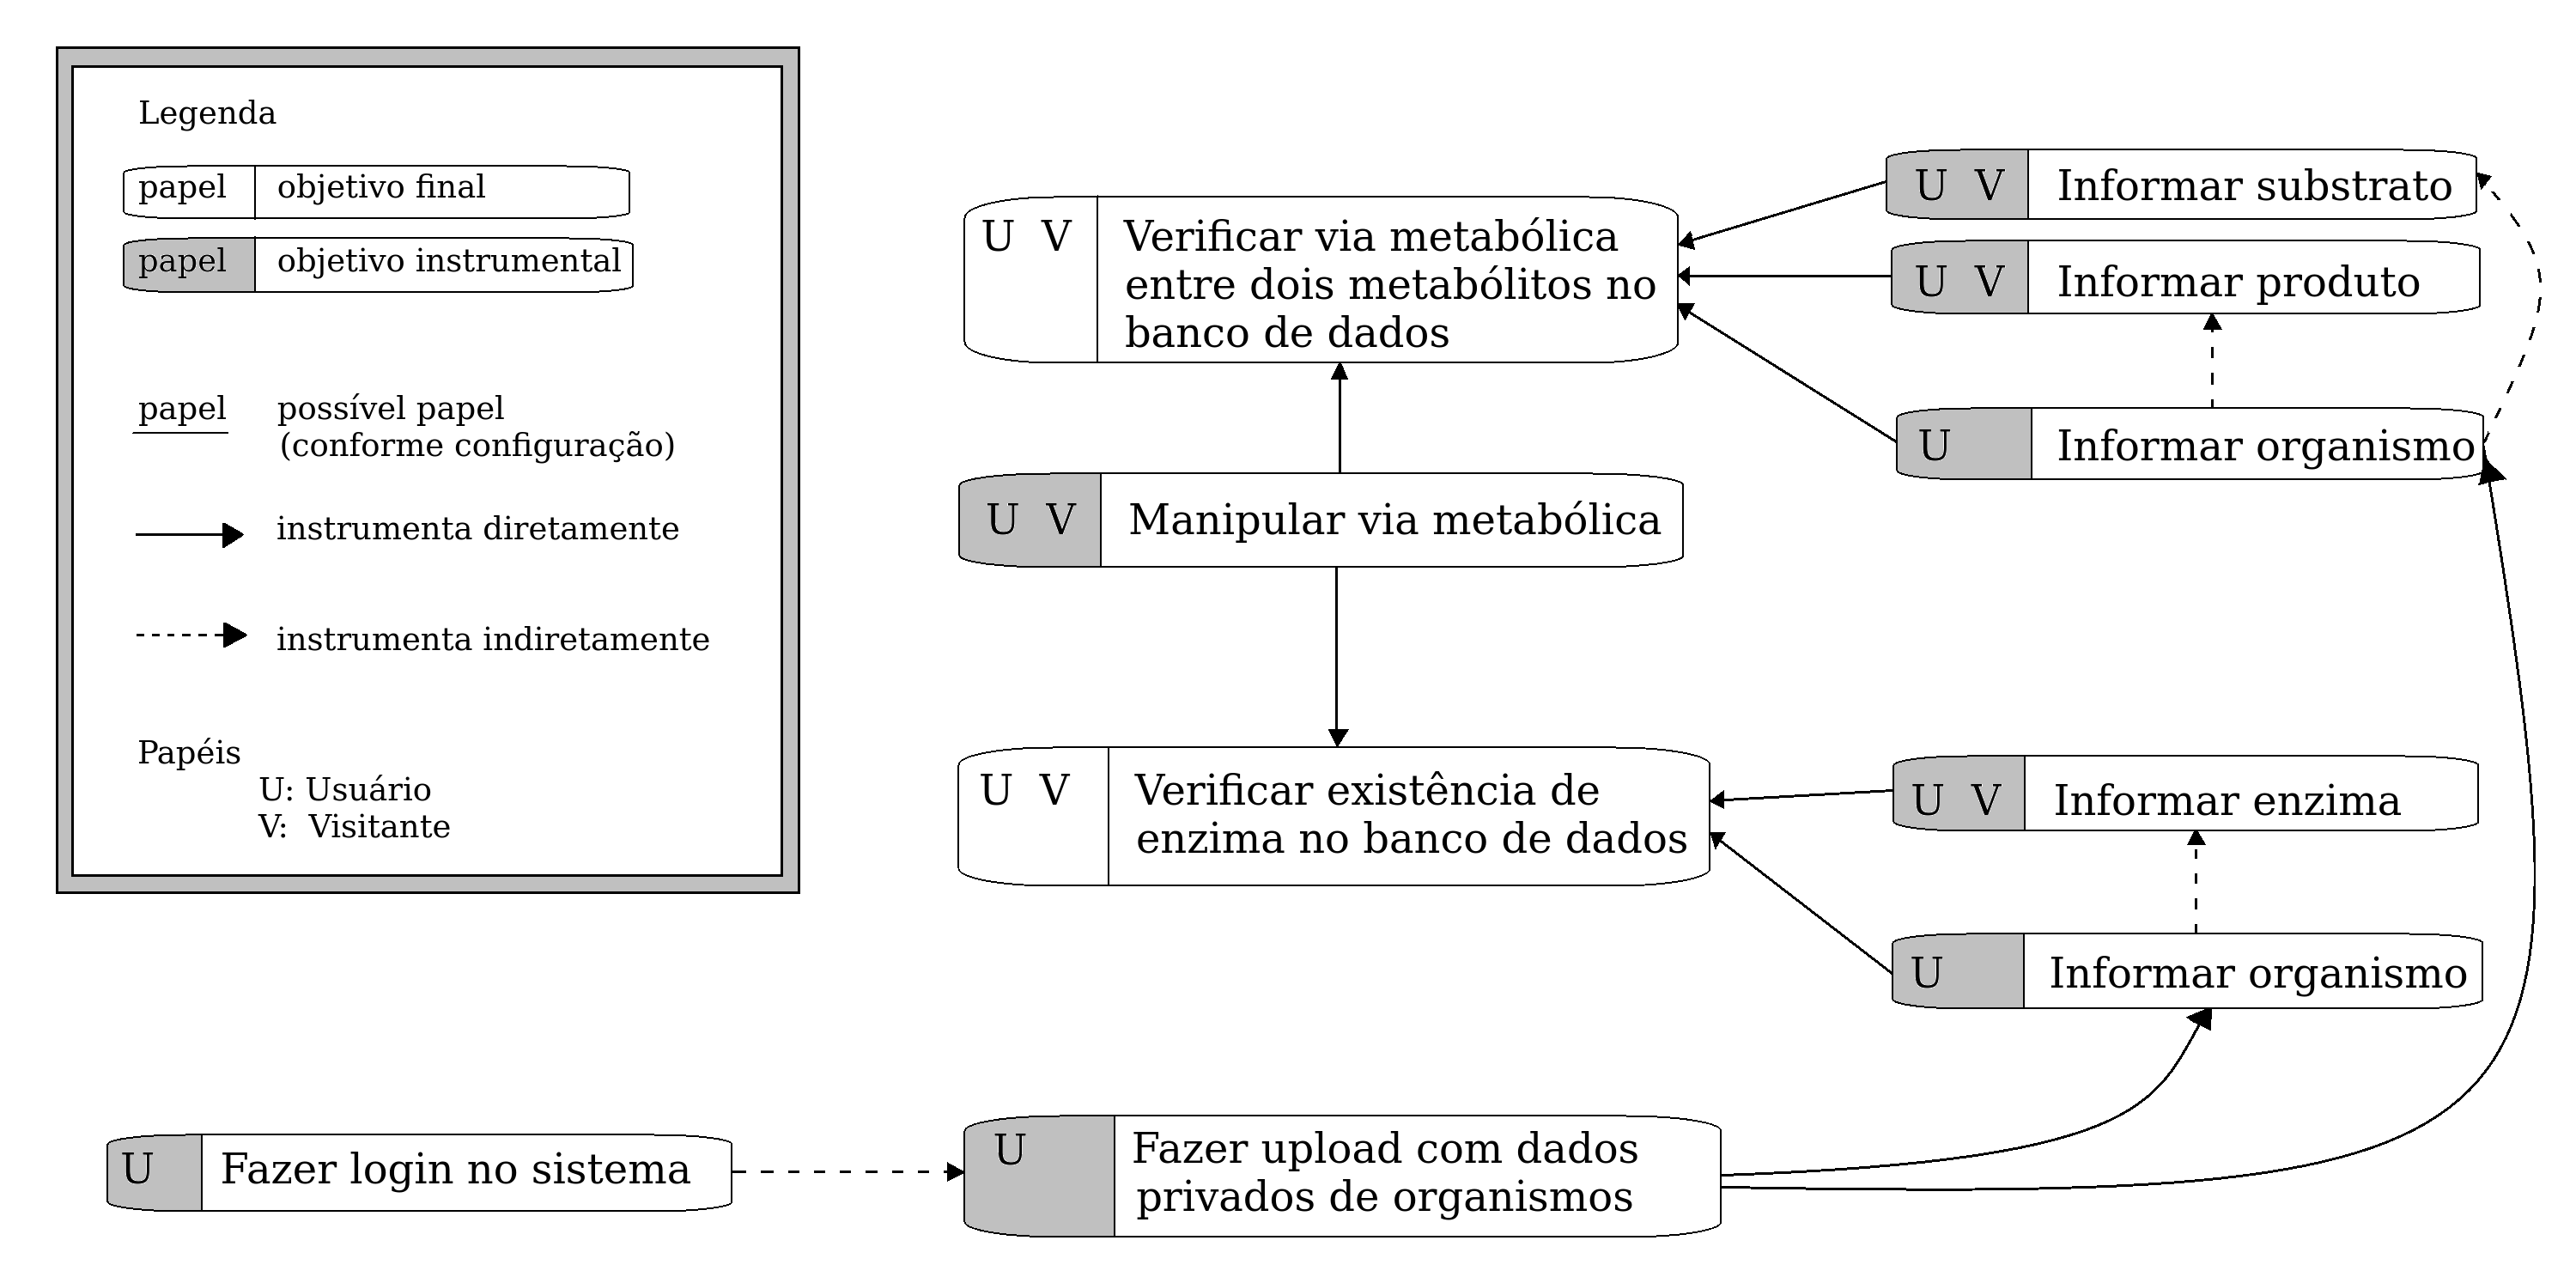
\includegraphics[width=1\textwidth]{mapaDeObjetivos.png}
    \caption{Mapa de Objetivos}
    \label{fig:mapaDeObjetivos}
\end{figure} 

\subsection{Modelagem de Tarefas}

\subsection{Tratamento de Rupturas na Comunicação}

\indent 
\begin{table}
\centering
\caption{Campos de entrada dos usuários do sistema 2Path} \label{prevencaoRecuperacao:2Path}
\begin{tabular}{|l|c|c|}
\hline
{\cellcolor[HTML]{DFDFDF}\textbf{Signo}} &  {\cellcolor[HTML]{DFDFDF}\textbf{Prevenção}} &  {\cellcolor[HTML]{DFDFDF}\textbf{Recuperação}}\\ \hline
\specialcell{Seleção de\\organismo}  & \specialcell{PA: Campo obrigatório para\\ formulários ``\textit{Search Enzyme}\\\textit{in Organism}'' e  ``\textit{Search}\\\textit{Pathway in Organism}''.\\Caso o usuário esqueça\\de selecionar este campo,\\o organismo escolhido será o\\primeiro em ordem alfabética.} & -  \\ \hline

\specialcell{Seleção de\\enzima} & \specialcell{PP: Campo obrigatório com\\indicador ``*''} & \specialcell{RA: Mensagem de texto em vermelho \\aparece acima do formulário informando\\o usuário de que o campo obrigatório\\não foi preenchido: ``\textit{Enzyme: Validation}\\\textit{ Error: Value is required}''.} \\ \hline

\specialcell{Seleção de\\substrato} & \specialcell{PP: Campo obrigatório com\\indicador ``*''} & \specialcell{RA: Mensagem de texto em vermelho \\aparece acima do formulário informando\\o usuário de que o campo obrigatório\\não foi preenchido: ``\textit{From: Validation}\\\textit{Error: Value is required.}''.\\O ``From'' significa que a via\\tem início neste metabólito} \\ \hline

\specialcell{Seleção de\\produto} & \specialcell{PP: Campo obrigatório com\\indicador ``*''} & \specialcell{RA: Mensagem de texto em vermelho \\aparece acima do formulário informando\\o usuário de que o campo obrigatório\\não foi preenchido: ``\textit{To: Validation}\\\textit{Error: Value is required.}''.\\O ``To'' significa que a via\\finaliza neste metabólito} \\ \hline
\end{tabular}
\end{table}

% =========================================================================================

\section{Detalhes de Implementação}


\indent O sistema desenvolvido para este projeto é uma aplicação web chamada \textit{2Path}. O usuário deve se cadastrar no \textit{website} para ter acesso às redes metabólicas do banco de dados do sistema, bem como pesquisar por palavras chaves no mesmo. Nesta seção serão apresentadas as linguagens e ferramentas utilizadas no desenvolvimento do \textit{website}, as características, funcionalidades e limites do sistema e, por fim, as dificuldades enfrentadas na implementação do projeto.

\indent O sistema foi desenvolvido no amibiente de desenvolvimento integrado \textit{open source} Eclipse Java EE - \textit{Java Platform, Enterprise Edition}, versão Mars 4.5.2. Para simplificar a obtenção das dependências do projeto, ou seja, pacotes de arquivos java (extensão .jar), foi utilizada o Apache Maven\footnote{\textit{Software} de gerenciamento de projeto e ferramenta de compreensão de programa.}. Este \textit{software} opera sobre o arquivo \textit{pom.xml}, onde POM significa \textit{Project Object Model} e contém as especificações de cada projeto que se tornará dependência do sistema em desenvolvimento, além de outros aspectos do código. O servidor selecionado para hospedagem local, \textit{localhost} porta 8080, do sistema foi o Apache TomCat versão 7.0.

\indent As páginas da aplicação foram desenvolvidas na linguagem de marcação XHTML, \textit{Extensible Hypertext Markup Language}, e a estilzação em CSS, \textit{Cascading Style Sheets}. Para conexão entre \textit{front-end} e \textit{back-end} foram utilizados JSF\footnote{Especificação Java para criação de componentes de interface de aplicação \textit{web}.}, Primefaces\footnote{Biblioteca com uma coleção de componentes de interface voltadas para JSF.}, e AngularJS, para a construção do grafo de vias metabólicas.

\indent JSF: \url{https://projetos.inf.ufsc.br/arquivos_projetos/projeto_1214/Ferramenta\%20de\%20mapeamento\%20de\%20UIDs\%20para\%20JSF.pdf}

\indent CORES: \url{http://www.hermancerrato.com/graphic-design/images/color-images/the-meaning-of-colors-book.pdf}, \url{http://www.awwwards.com/trendy-web-color-palettes-and-material-design-color-schemes-tools.html}, \url{https://medium.com/wdstack/how-the-bootstrap-grid-really-works-471d7a089cfc#.k7w39z2uh}

% Communication websites which market to individual customers on a one-to-one basis would benefit with some blue in their marketing. Hi-tech and computer technology businesses can benefit from most shades of blue combined with gray.

\subsection{Banco de Dados OrientDB}

\indent O banco de dados escolhido para armazenar as enzimas, compostos, reações e demais elementos foi o OrientDB.\\
CITAR: (1) Graph database, (2) SQL, (3) Commercial Friendly License, (4) Low Total Cost of Ownership (TCO) Community Edition, (5) Open Source. \url{http://orientdb.com/why-orientdb/}, \url{http://orientdb.com/docs/last/Java-API.html}

\subsection{Desafios}
 
O que foi o trabalho. 
Decrever todo o ambiente usado
Neste capítulo serão apresentados os primeiros resultados experimentais obtidos.
  \chapter{Resultados dos testes}

\indent Neste capítulos serão apresentados os resultados dos testes realizados seguindo o protocolo do Método de Avaliação de Comunicabilidade. A Seção \ref{avaliacaoDeInterface} descreve o perfil dos usuários, a análise dos vídeos, a interpretação dos vídeos e etiquetagem do \textit{feedback} dos usuários e, por fim, o perfil semiótico do sistema. Esse perfil tem o objetivo de auxiliar na implementação da nova proposta de interface, descrita também nessa seção. A Seção \ref{novaInterface} apresenta as mudanças feitas na interface antiga, bem como as modificações feitas e decisões de projeto para a nova proposta de interface.

\section{Avaliação da Interface} \label{avaliacaoDeInterface}

\indent Os testes foram realizados com 3 biólogos, identificados aqui como Usuário 1, 2 e 3, respectivamente. O fato de a avaliação ser qualitativa, e não quantitativa, explica o baixo número de usuários participantes dos testes. A Tabela \ref{dados_pessoais} apresenta os dados pessoais de cada um, levando em consideração, principalmente, a experiência que já possuem em redes metabólicas. Isso é necessário, pois quanto mais eles conhecem sobre o conteúdo, mais críticos são a respeito da interface com a qual devem interagir em seu trabalho e pesquisas.

\begin{table}[h!]
  \centering
  \caption{Conhecimento dos biólogos selecionados para o teste a respeito dos conceitos utilizados no desenvolvimento da interface do 2Path}
  \label{dados_pessoais}
  \begin{tabular}{lccc}
  & Usuário 1 & Usuário 2 & Usuário 3 \\ \hline
  {\cellcolor[HTML]{DFDFDF}\specialcell{Formação\\acadêmica}} & Possui pós-doutorado & Possui mestrado & Possui metrado \\ \hline
  {\cellcolor[HTML]{DFDFDF}\specialcell{Bancos de\\dados biológicos}} & Conhece bastante & Nunca utilizou  & Conhece \\ \hline
  {\cellcolor[HTML]{DFDFDF}\specialcell{Redes\\metabólicas}} & Conhece bastante & Nunca utilizou & Nunca utilizou  \\ \hline
  {\cellcolor[HTML]{DFDFDF}\specialcell{Ferramentas\\de visualização\\de redes\\metabólicas}} & Conhece bastante & Nunca utilizou  & Nunca utilizou  \\ \hline
  \end{tabular}
\end{table}

\indent Após preencherem o questionário de dados pessoais e conhecimentos do conteúdo a serem expostos, do Apêndice \ref{questionario_dados_pessoais}, os biólogos iniciaram as tarefas propostas pelo avaliador, descritas no Apêndice \ref{tarefas}. A seguir são listadas todas as principais evidências implícitas e explícitas de falha de comunicação dos usuários 1, 2 e 3 com a interface, nas Tabelas \ref{usuario1}, \ref{usuario2} e \ref{usuario3} , respectivamente. Elas estão ordenadas pelo tempo em que aparecem nos vídeos.

\begin{table}[h!]
	\centering
	\caption{Análise do usuário 1. Duração: 10 minutos e 44 segundos.}
	\label{usuario1}
	\begin{tabular}{|cl|}
	\hline
	Tempo & Ação do usuário. \\ \hline
	(01:22) & \specialcell{Usuário não encontrou as reações que a enzima catalisa, mas logo\\percebeu que deveria seguir para uma outra página para obter\\detalhes sobre a busca} \\ \hline
	(01:26) & \specialcell{Usuário se deparou com um grafo em movimento, com 6 nós e cinco arestas,\\e não entendeu seu significado, a princípio} \\ \hline
	(01:55) & \specialcell{Usuário interagiu com o grafo forçado, pois o mesmo não parava de se mover} \\ \hline
	(03:50) & \specialcell{Usuário diz "Nossa, isso é muito ruim; Não dá pra saber se o substrato da\\enzima é verde (Composto) ou o rosa (Reação)"} \\ \hline
	(05:10) & \specialcell{Usuário tenta entender a legenda do grafo, mas discorda totalmente do\\proposto} \\ \hline
	(07:49) & \specialcell{Usuário não encontra informação que buscava, até descobrir que deveria\\seguir para página de detalhes de busca, novamente} \\ \hline
	(07:53) & \specialcell{Usuário expressa desgosto pelo grafo fechado que aparece ao iniciar a página\\de detalhes da via metabólica} \\ \hline
	(08:59) & \specialcell{Usuário esqueceu de selecionar \textit{Search} e percebeu que havia selecionado\\em ver detalhes da busca anterior} \\ \hline
	(10:15) & \specialcell{Usuário logo clica no grafo para ele parar de se mover} \\ \hline
	\end{tabular}
\end{table}

\begin{table}[h!]
	\centering
	\caption{Análise do usuário 2. Duração: 11 minutos e 08 segundos.}
	\label{usuario2}
	\begin{tabular}{|cl|}
		\hline
		Tempo & Ação do usuário. \\ \hline
		(00:41) & \specialcell{Usuário percebeu que havia selecionado um botão que não o levava ao seu\\objetivo} \\ \hline
		(01:29) & \specialcell{Usuário se confunde com função \textit{auto-complete} do campo de enzimas} \\ \hline
		(02:01) & \specialcell{Usuário demora alguns segundos para perceber que deve seguir para a página\\de detalhes de busca} \\ \hline
		(02:20) & \specialcell{Usuário demora alguns segundos para entender, a partir da legenda, o\\significado do grafo que aparece na página de detalhes de busca} \\ \hline
		(04:55) & \specialcell{Usuário não percebe que página retornou sucesso, pois a aparência é de que\\a mesma não foi atualizada, uma vez que o resultado da busca atual é o\\mesmo que a busca anterior} \\ \hline
		(07:55) & \specialcell{Usuário tenta impedir grafo de se mover para fora de seu campo de visão} \\ \hline
		(08:18) & \specialcell{Usuário tem dificuldade para entender significado biológico do grafo} \\ \hline
		(09:26) & \specialcell{Usuário esqueceu de selecionar \textit{Search} e percebeu que havia selecionado\\em ver detalhes da busca anterior} \\ \hline
		(10:01) & \specialcell{Usuário tenta impedir grafo de se mover para fora de seu campo de visão} \\ \hline
		(10:45) & \specialcell{Usuário percebeu que havia errado a tarefa anterior e voltou para refazê-la} \\ \hline
	\end{tabular}
\end{table}

\begin{table}[h!]
	\centering
	\caption{Análise do usuário 3. Duração: 7 minutos e 49 segundos.}
	\label{usuario3}
	\begin{tabular}{|cl|}
		\hline
		Tempo & Ação do usuário. \\ \hline
		(01:05) & \specialcell{Usuário se confunde com função \textit{auto-complete} do campo de enzimas. Ainda\\percebe que o problema não é o teclado, mas sim a função que aparece\\sem necessidade e atrapalha a busca} \\ \hline
		(01:46) & \specialcell{Usuário diz "É só essa a informação?", pois não percebeu, a princípio, que\\para realizar a tarefa deveria seguir para a página de detalhes da busca} \\ \hline
		(01:59) & \specialcell{Usuário não entende grafo que aparece na tela de detalhes e reclama muito\\por ele não estar inicialmente parado} \\ \hline
		(04:20) & \specialcell{Usuário reclama da falta de respostas da interface} \\ \hline
		(06:00) & \specialcell{Usuário acha um absurdo o tamanho do grafo que aparece na tela e pede\\a lista dos detalhes que ele gostaria de saber sobre a busca} \\ \hline
		(07:20) & \specialcell{Usuário reclama da falta de respostas da interface} \\ \hline
		(07:25) & \specialcell{Usuário acha um absurdo o tamanho do grafo que aparece na tela e pede\\a lista dos detalhes que ele gostaria de saber sobre a busca} \\ \hline
	\end{tabular}
\end{table}


\subsection{Interpretação dos Resultados}

\indent A etiquetagem foi realizada seguindo os padrões da fase de interpretação de dados do Método de Avaliação de Comunicabilidade, descrito no capítulo 2. As etiquetas são apresentadas na Tabala \ref{tabela_de_etiquetas}.

\begin{table}[h!]
  \centering
  \caption{Contabilização das etiquetas para cada usuário. Cada etiqueta é registrada no tempo do vídeo em que ela ocorreu.}
  \label{tabela_de_etiquetas}
  \begin{tabular}{|l|c|c|c|}
  \hline
  {\cellcolor[HTML]{DFDFDF}Etiqueta} & {\cellcolor[HTML]{DFDFDF}Usuário 1} & {\cellcolor[HTML]{DFDFDF}Usuário 2} & {\cellcolor[HTML]{DFDFDF}Usuário 3} \\ \hline
  Desisto. & - & - & - \\ \hline
  Para mim está bom... & - & - & - \\ \hline
  Não, obrigado. & - & - & - \\ \hline
  Vai de outro jeito. & - & - & - \\ \hline
  Cadê? & (01:22), (07:49) & (04:55) & - \\ \hline
  Ué, o que houve? &  & - & - \\ \hline
  E agora? & - & (02:01) & (01:46) \\ \hline
  Onde estou? & - & - & - \\ \hline
  Epa! & (08:59) & \specialcell{(00:41), (09:26),\\(10:45)} & - \\ \hline
  Assim não dá. & (5:10) & (01:29) & (01:05) \\ \hline
  O que é isto? & (01:26), (03:50) & (02:20), (08:18) & (01:59) \\ \hline
  Socorro! & \specialcell{(01:55), (07:53),\\(10:15)} & (07:55), (10:01) & (06:00), (07:25) \\ \hline
  Por que não funciona? & - & - & (04:20), (07:20) \\ \hline
  \end{tabular}
\end{table}

\indent Após a realização das tarefas, cada biólogo respondeu a um questionário, do Apêndice \ref{questionario_interface}, para que fosse avaliado também sua opinião a respeito do sistema.

\indent O usuário 1 relatou que, apesar de as tarefas serem relativamente fáceis, a representação das vias metabólicas é confusa, pois a reação é uma ação, portanto seria melhor representada como uma aresta. Quem recebe o substrato e produz outro composto a partir desse é a enzima, portanto o grafo deveria ser configurando mantendo essa informação biológica. Foi reportado, também, que a legenda do grafo estava confusa e poderia conter apenas informações sobre os nós, removendo as informações sobre as arestas, que são óbvias para os biólogos. Por fim, o usuário 1 sugeriu que a via metabólica aparecesse inicialmente estática e com os nós distantes uns dos outros.

\indent O usuário 2 relatou que as tarefas foram fáceis de serem realizadas e didáticas. Segundo ele, praticamente todos os elementos da interface estavam claros, com exceção do grafo, uma vez que entendeu que as reações eram arestas.

\indent Por fim, o usuário 3 relatou que as tarefas foram difíceis de serem realizadas, principalmente a segunda, de pesquisar por vias metabólicas entre dois compostos. Na primeira tarefa, o teclado numérico e a função \textit{auto-complete} diminuíram a usabilidade da interface. Já na segunda tarefa, ele seguiu por um caminho diferente do esperado sem perceber, e acidentalmente descobriu um erro no sistema, que retornava dois grafos ao invés de um só. Para justificar seu erro de navegação, ele relatou que não havia percebido a seção de busca no banco de dados completo, à esquerda da página de busca. Além disso, assim como o usuário 1, ele sugeriu que a via metabólica aparecesse inicialmente estática e com os nós distantes uns dos outros.

\subsection{Consolidação dos resultados}

\indent A partir das análises dos três biólogos, foram verificados vários pontos fracos no sistema. Como foram observadas várias falhas de comunicação na interface proposta, foi mais adequado apresentá-las em forma de lista do que em forma de resposta às perguntas da fase de consolidação de usuário, do Método de Avaliação de Comunicabilidade.

\indent De maneira geral, os usuários conseguiram realizar seus objetivos, porém de maneira ineficiente e geralmente errando ao tentar pela primeira vez. Vários elementos da interface deixaram os usuários insatisfeitos e desmotivados a continuar a tarefa. Os problemas se manifestam principalmente na área de visualização do grafo que representam as vias metabólicas. Houveram elogios, apesar das barreiras de comunicação. Várias páginas possuíam textos explicativos, que os usuários leram e, além disso, a função de \textit{auto-complete} dos nomes dos compostos químicos foi de grande ajuda. A lista de falhas de comunicabilidade a seguir fornece a base de informação para a criação do perfil semiótico do sistema, assim como descrito no capítulo 2.

\begin{itemize}
\item Busca por enzima / via metabólica
  \begin{itemize}
  \item[1] O botão de voltar uma página, do navegador, não fazia o que o usuário esperava. Ele voltava para a pesquisa anterior em vez de ir para a página central de buscas;
  \item[2] A função \textit{auto-complete} das enzimas não foi uma boa decisão de projeto, pois os usuários ficavam confusos com os números que apareciam;
  \item[3] Resultado de busca não estava sendo inicializado sempre que página é carregada, portanto apresentava um resultado anterior, o que causava confusão;
  \item[4] Botão \textit{View Interative Data}, para visualizar a via metabólica, está sempre ativo. Isso fez com que os usuários não notassem que existe informação extra sobre enzima ou via quando a pesquisa retorna sucesso;
  \item[5] Botões \textit{Search} e \textit{View Interative Data} estavam muito próximos um do outro. Usuários às vezes não selecionavam o botão \textit{Search} antes de clicar em \textit{View Interative Data}, pois a segunda coluna da página estava mal localizada, para um formulário;
  \item[6] A página de busca central dá mais foco em busca por elementos no organismo, e isso faz com que a seção menor à esquerda passe despercebida.
  \end{itemize}

\item Visualização do grafo
  \begin{itemize}
  \item[1] A reação não deveria ser representada por um nó, pois para os biólogos, ela é uma ação, e não um elemento. Assim, faz mais sentido biológico uma aresta saindo do substrato para a enzima, e saíndo da enzima para o produto. A aresta entre enzima e reação não é necessária. Houve muita confusão, pois pensaram que reação era representada por aresta em vez de por um nó;
  \item[2] Não é necessário apresentar os nós do organismo e sequências que o organismo possui. Ao apresentar a enzima na busca de informações no organismo, já é implícito que aquela enzima é produzida pelo organismo;
  \item[3] Quanto maior o grafo, mais complexo é entendê-lo;
  \item[4] Grafos muito grandes podem ficar cortados e alguns elementos podem sair do campo de visão do usuário;
  \item[5] É mais desejável um grafo que apareça primeiramente de maneira estática. Um grafo que aparece se movendo levemente é irritante. Caso o usuário queira mover e clicar nos elementos, ele o faz com mais facilidade com um grafo estático;
  \item[6] É mais agradável um grafo que apareça aberto;
  \item[7] A legenda poderiam apresentar apenas informação a respeito dos nós, pois informações sobre as arestas são desnecessárias para os biólogos.
  \end{itemize}
\end{itemize}

\indent Alguns ítens lista de falhas de comunicabilidade podem ser verificados nas Figuras \ref{fig:falha_search_page}, \ref{fig:falha_search_enzyme} e \ref{fig:falha_graph}. A primeira apresenta as dificuldades enfrentadas na página geral de buscas. A Figura segunda apresenta as dificuldade enfrentadas na interface de busca por enzimas. Por fim, a terceira figura apresenta as falhas de comunicabilidade em relação à interface da via metabólica e do próprio grafo em si.

\indent Além dessas dificuldades relatadas, foi encontrado um erro de implementação em um dos testes. Uma das tarefas era encontrar uma via metabólica entre dois compostos no grafo completo do 2Path, porém um dos usuários utilizou a busca por via em um organismo. A busca deveria retornar que não há via, porém ela retornou que existia, e apresentou um grafo disjunto\footnote{Dois grafos que não se conectam.}. Um grafo era do organismo com todas as enzimas que ele produzia e o outro grafo representava a via entre os compostos pesquisados.

\newpage

\begin{figure}[!h]
	\centering
	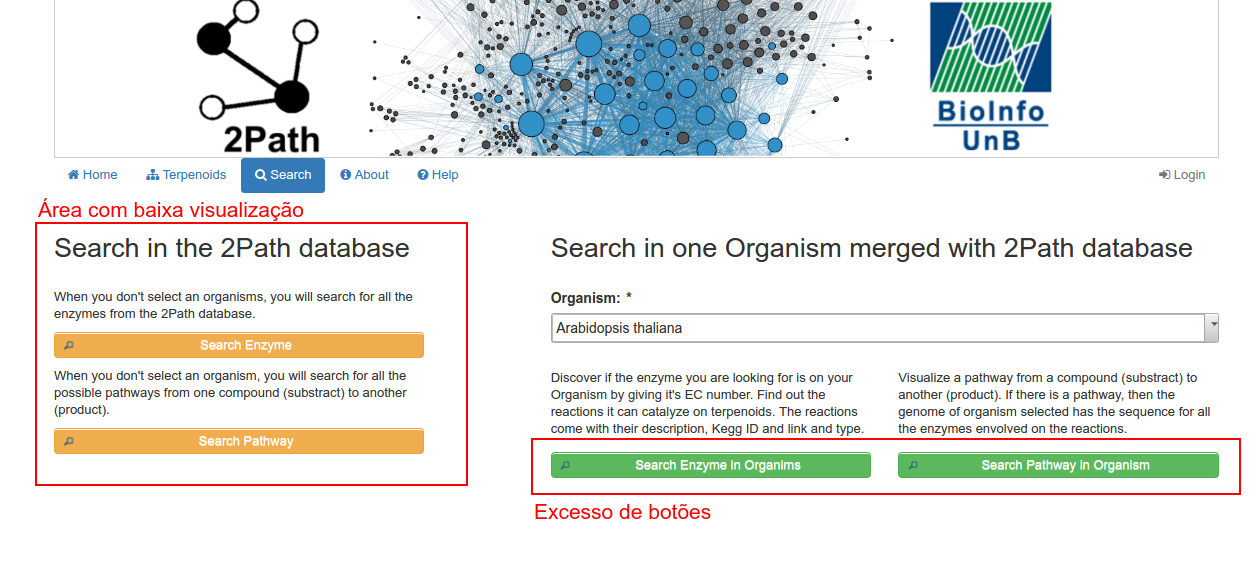
\includegraphics[width=1\textwidth]{falha_search_page.png}
	\caption{Falhas de comunicação na página de buscas gerais.}
	\label{fig:falha_search_page}
\end{figure}

\begin{figure}[!h]
	\centering
	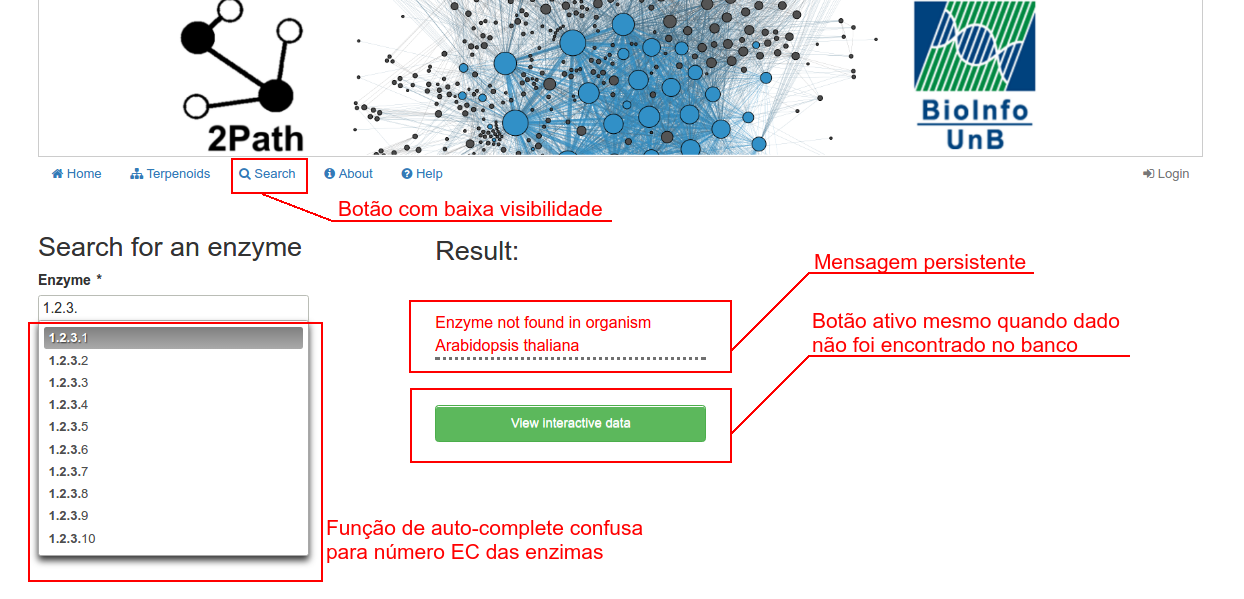
\includegraphics[width=1\textwidth]{falha_search_enzyme.png}
	\caption{Falhas de comunicação na página de busca por enzima em organismo.}
	\label{fig:falha_search_enzyme}
\end{figure}

\newpage

\begin{figure}[!h]
	\centering
	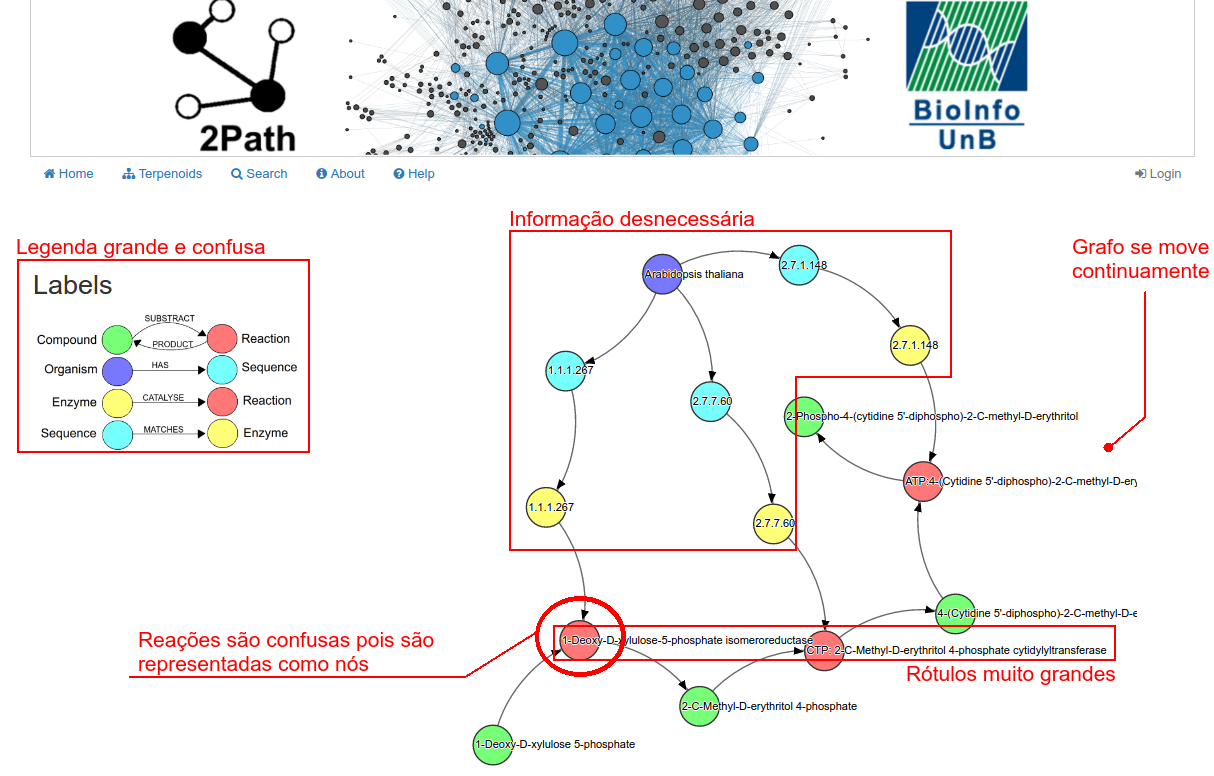
\includegraphics[width=1\textwidth]{falha_graph.png}
	\caption{Falhas de comunicação na página de visualização de via metabólica em organismo.}
	\label{fig:falha_graph}
\end{figure}

\indent Assim sendo, foi criado, a partir da análise completa dos dados, o seguinte perfil semiótico para a proposta de interface para o banco de dados 2path:

\begin{quote}
	Este é o meu entendimento, como projetista, de quem você, pesquisador biólogo, é, do que aprendi que você precisa buscar e visualizar, de maneira prática e com bastante \textit{feedback} legível, pois as informações podem ser extensas e complexas. A nova interface do 2Path, portanto, é o sistema que projetei para você, e a busca vinculada à visualização das vias metabólicas e enzimas é a forma como você pode utilizá-lo para alcançar uma gama de objetivos que se encaixam nesta visão.
\end{quote}

\indent O perfil semiótico descrito, bem como a lista de barreiras de comunicação entre projetista e usuário, exerceram papel de guia para o desenvolvimento da nova proposta de interface do 2path. A seguir está uma lista de mudanças no projeto de interface, feita após os testes do Método de Avaliação de Comunicabilidade. Cada item representa a solução dos problemas relatados na lista anterior, de falhas de comunicabilidade.

\begin{itemize}
\item Busca por enzima / via metabólica
  \begin{itemize}
  \item[1] Foi adicionado um botão de voltar nas páginas específicas de busca por enzima e vias metabólicas, assim o usuário pode clicar nele e voltar diretamente para a página de buscas gerais;
  \item[2] A função \textit{auto-complete} do campo de busca por enzima foi removida;
  \item[3] As mensagens de sucesso e erro são apresentadas no canto superior direito da tela e são atualizadas sempre que uma nova busca é feita. Ela aparece por 5 segundos e depois desaparece;
  \item[4, 5] O grafo que apresenta os detalhes sobre a enzima ou via metabólica buscada aparece na mesma página que o formulário de pesquisa. Se a busca retorna verdadeira, o grafo aparece, se retorna falsa, não aparece. Assim, o usuário não precisa seguir mais um passo na interface para visualizar os dados biológicos que procura;
  \item[6] As colunas de busca no banco completo e no organismo foram configuradas com o mesmo tamanho. Os ícones que simbolizam elementos públicos e privados foram posicionados ao lado dos títulos das buscas no banco completo e em organismos, respectivamente.
  \end{itemize}
  
\item Visualização do grafo
  \begin{itemize} 
  \item[1] Representar as reação com a \textit{label} das enzimas não é possível, pois o banco de dados não possui suporte para a obtenção dessa informação. Além disso, uma enzima pode catalisar mais de uma reação. Assim, não teria como representar apenas um nó da enzima recebendo todos os possíveis substratos e produzindo todos os possíveis produtos. Uma solução para esse problema seria solicitar ao administrador do \textit{2Path} a adição de mais uma propriedade no nó da reação que determine a enzima que a catalise;
  \item[2, 3, 4] Para diminuir o tamanho do grafo, foram omitidos os nós referentes ao organismo e às sequências do genoma que ele possui;
  \item[5] O grafo aparece estático, porém o usuário pode clicar nos nós e movê-los como desejar;
  \item[6] Os nós do grafo não se sobrepõem, portanto ele tem a aparência de que está aberto;
  \item[7] A legenda apresenta apenas informações sobre as cores de três nós: Compostos, Reações e Enzimas.
  \end{itemize}
\end{itemize}
 
 

\section{Nova Interface do 2Path} \label{novaInterface}

\indent Na nova proposta de interface para o 2Path, as páginas de \textit{Home}, \textit{Terpenoids} e \textit{About} continuam as mesmas. Na página de \textit{Help} foram trocadas apenas as figuras ilustrativas que auxílio a navegação no sistema. As grandes mudanças ocorreram na página de \textit{Search}, na busca por enzimas e vias metabólicas.

\indent A página principal de busca anterior possui duas colunas principais, a da esquerda destinada à buscas por enzimas e vias metabólicas no banco de dados completo do 2Path, e a da direita, destinada à busca em um organismo específico. Como o organismo era do próprio usuário, optou-se por deixar a coluna da direita duas vezes maior que a da esquerda, mas essa decisão de interface acabou ofuscando a busca no banco completo. A interface também era um pouco confusa, pois existiam quatro botões e muito texto.

\indent Na nova interface da página principal de busca, existe apenas uma coluna à esquerda e um campo onde o usuário pode selecionar a busca no banco completo ou em um de seus organismos. Nesse sentido, são necessários apenas dois botões, um de busca por enzima e outro de busca por via metabólica. A Figura \ref{fig:new_search_page} apresenta a página descrita.

\begin{figure}[!h]
    \centering
    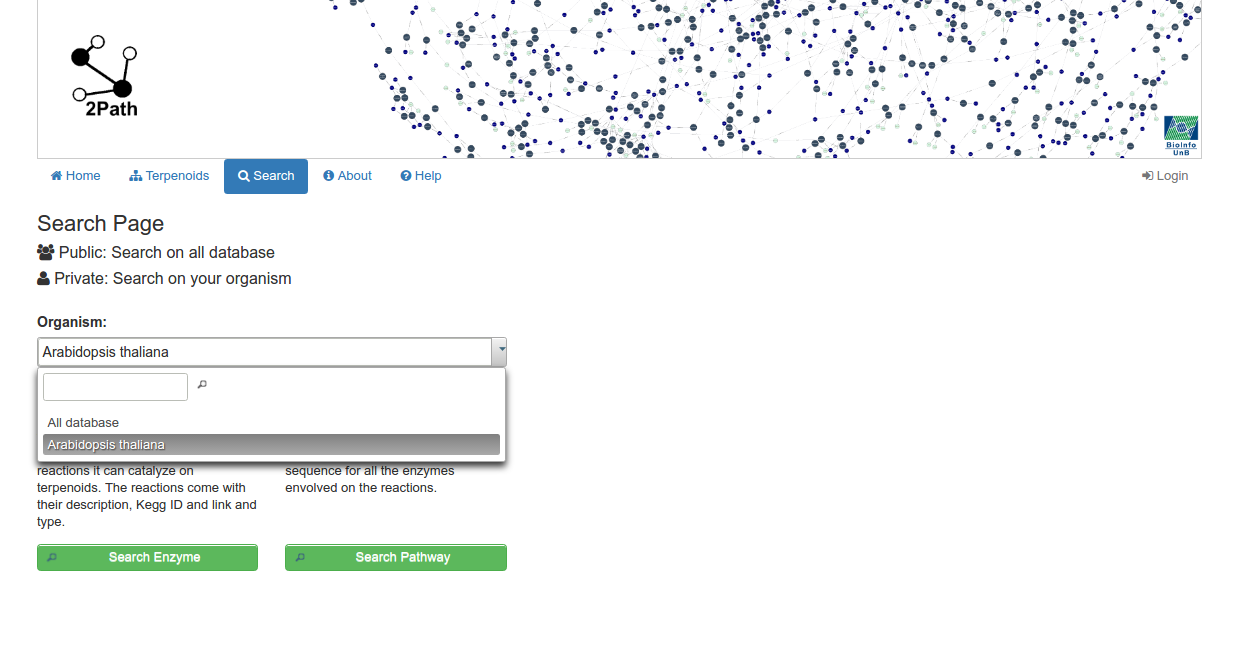
\includegraphics[width=1\textwidth]{new_search_page.png}
    \caption{Nova interface da página principal de buscas.}
    \label{fig:new_search_page}
\end{figure}

\indent A antiga interface para buscar por enzima possuía duas páginas, nas quais o objetivo da primeira era relatar se a enzima existe no banco de dados e o objetivo da segunda era de apresentar o grafo da enzima e as reações que catalisava, se existisse. Essa interface, porém era bastante confusa, principalmente os \textit{feedbacks} dados na busca, pois não atualizavam corretamente. A função de \textit{auto-complete} do EC das enzimas também diminuiu a usabilidade, pois acredita-se que não seja natural um campo de entrada completar números. Além disso, quando o usuário seguia para a página de visualização dos dados biológicos, eles precisavam clicar e arrastar os nós de maneira forçada, pois os mesmos não paravam de se mexer. O objetivo era apresentar um grafo simples e interativo, porém a experiência de usuário não correspondeu ao esperado.

\indent A nova interface para busca de enzima sofreu fortes mudanças. Não há mais função de \textit{auto-complete} no campo de entrada de EC, foi adicionado um botão para retornar à página de busca e, principalmente, o grafo aparece na mesma página. Se existe enzima, o grafo aparece, se não existe, não aparece. Os rótulos dos nós, que antes apresentavam seus nomes, agora apresenta seus identificadores no KEGG. Acima do grafo está uma legenda que aparece quando o usuário passa o \textit{mouse} por cima dos nós. Ela possui informações sobre o tipo do nó, seu nome e seu identificador no KEGG. Este nó é destacado por uma cor mais escura que os demais.

\indent A Figura \ref{fig:new_enzyme_4_catalyses}, além de apresentar a nova interface, mostra que não é possível representar as reações como enzimas, pois uma enzima pode catalisar mais de uma reação. Se as próprias reações possuíssem informação sobre qual enzima as catalisam, então essa mudança seria possível. Essa alteração no banco de dados facilitaria bastante a interpretação do grafo, de acordo com os biólogos, que costumaram entender reação como aresta. Por fim, a legenda do grafo ficou mais simples, portanto, mais legível.

\begin{figure}[!h]
	\centering
	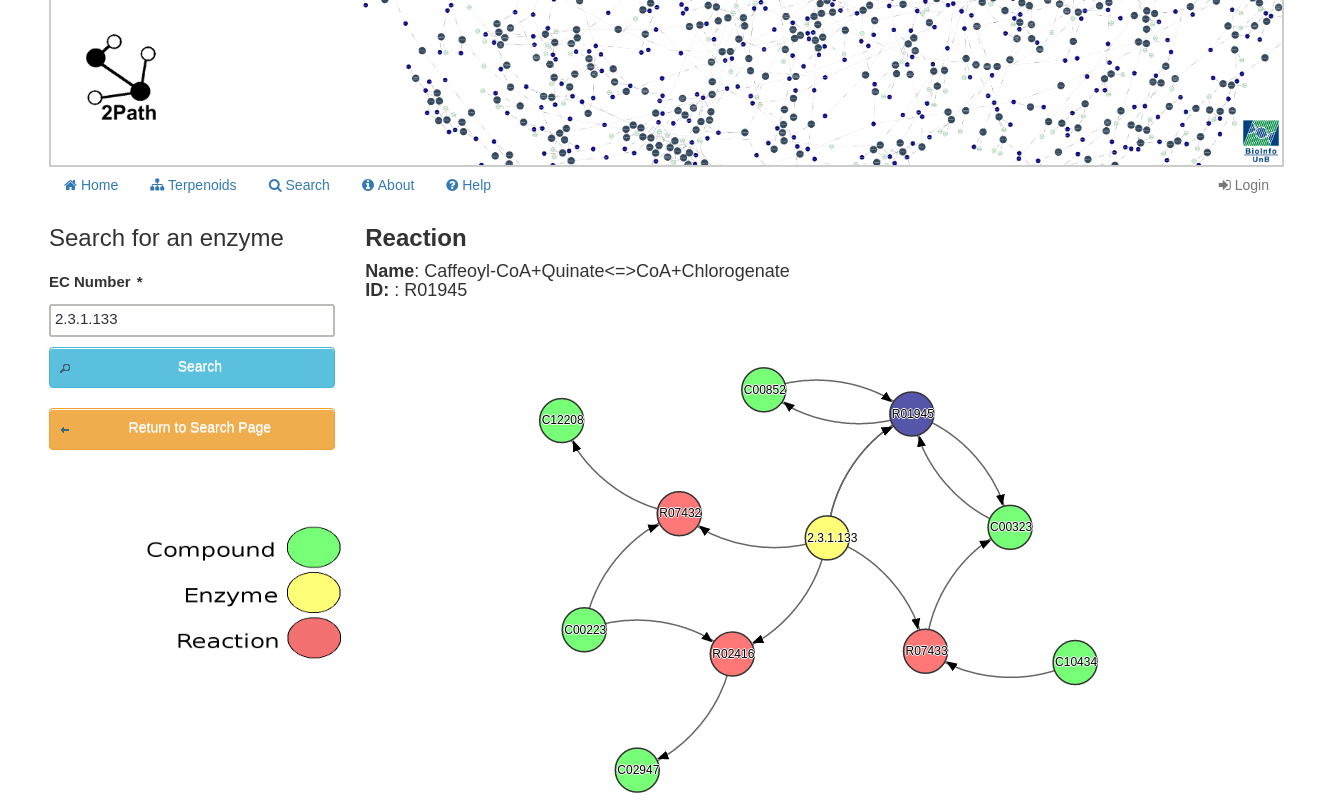
\includegraphics[width=1\textwidth]{new_enzyme_4_catalyses.png}
	\caption{Nova interface da página de busca por enzima, tanto em um organismo quanto no banco de dados completo. Nesta interface, o usuário passou o mouse por cima do nó \textit{R01945}, que foi destacado de cor escura, e seus detalhes foram exibidos acima do grafo.}
	\label{fig:new_enzyme_4_catalyses}
\end{figure}

\indent Em relação à busca por vias metabólicas, a nova interface se assemelha com a de busca por enzima, porém continua com a função de \textit{auto-complete} nos campos de entrada por nome de compostos, que foi uma boa decisão de projeto. A Figura \ref{fig:new_message_success} apresenta o resultado da busca pela via entre \textit{Caffeate} e \textit{Chlorogenate}. Observa-se que retornou sucesso, pois além de a via ter aparecido na tela, uma mensagem de sucesso aparece, por 5 segundos, no canto superior direito da tela.

\begin{figure}[!h]
    \centering
    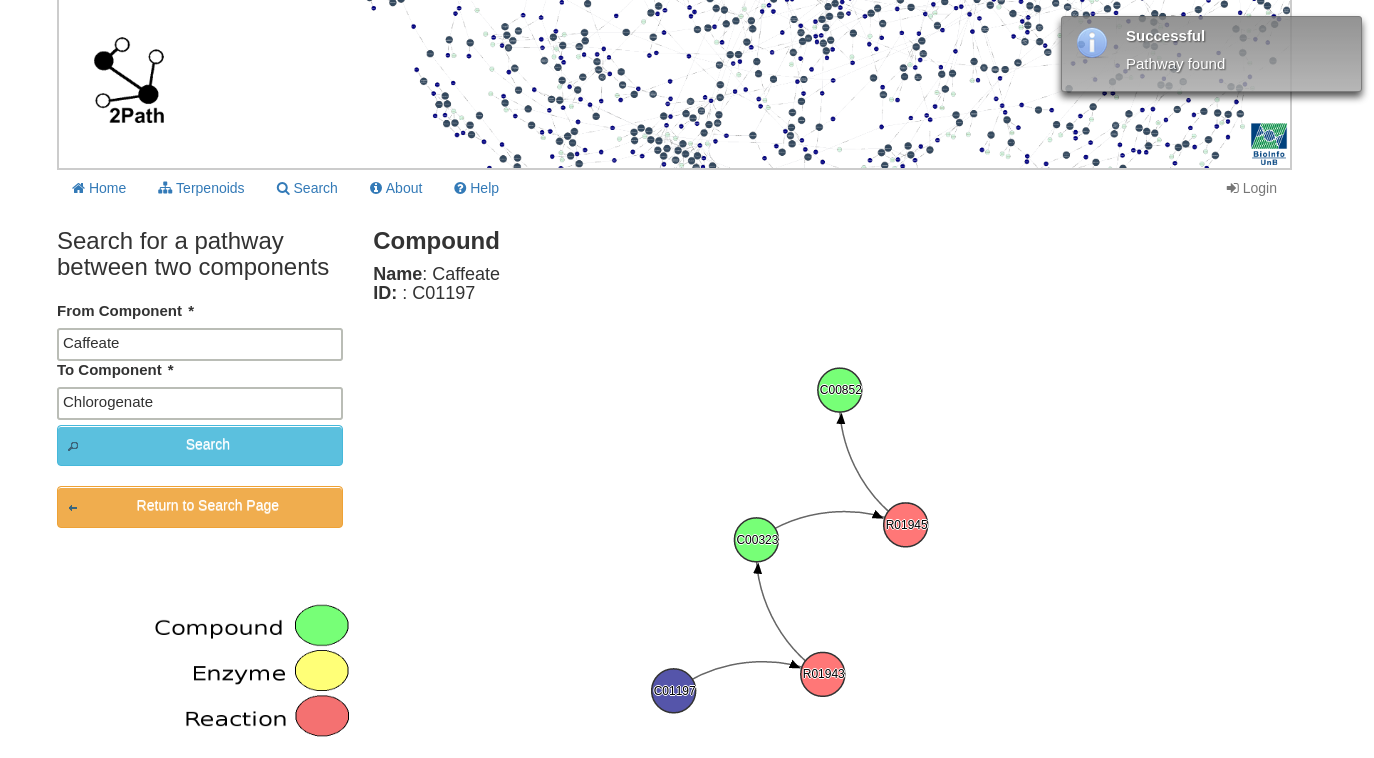
\includegraphics[width=1\textwidth]{new_message_success.png}
    \caption{Nova interface da página de busca por via metabólica, tanto em um organismo quanto no banco de dados completo. Nesse caso, a busca retornou sucesso no banco de dados completo do 2Path.}
    \label{fig:new_message_success}
\end{figure}


\indent As Figuras \ref{fig:new_message_error} e \ref{fig:new_pathway} aprensentam resultados de busca por via metabólica em um organismo. A primeira retornou falso, como visto pela mensagem de erro. A segunda retornou mensagem de sucesso e um grafo estático na tela. Observe que, apesar de a busca ter sido no organismo, a única informação que interessa para o usuário é da via entre um composto e outro. Portanto não aparecem mais como na interface antiga os nós do organismo, sequências e enzimas. Acredita-se que essa nova decisão de projeto diminui a complexidade da visualização dos dados biológicos.


\begin{figure}[!h]
    \centering
    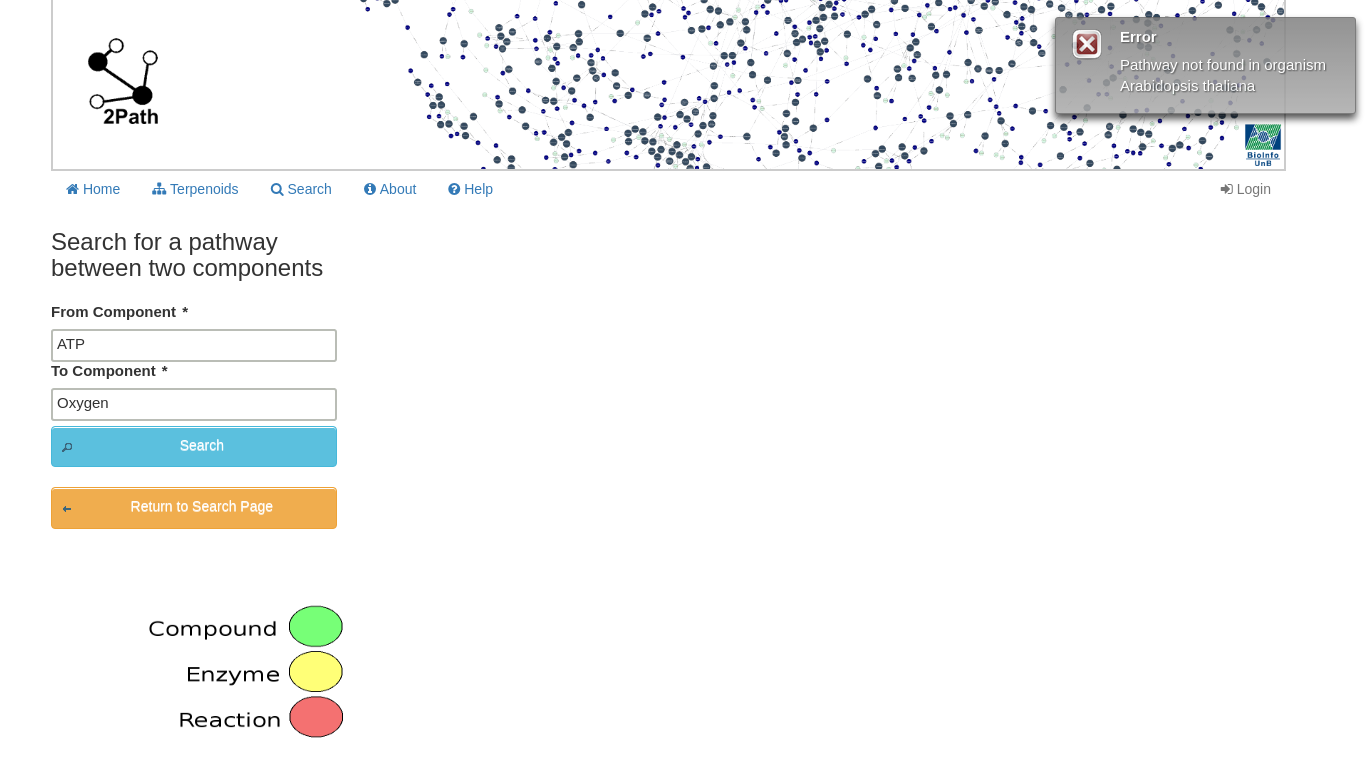
\includegraphics[width=1\textwidth]{new_message_error.png}
    \caption{Nova interface de busca por via metabólica quando a busca retorna erro de via não encontrada.}
    \label{fig:new_message_error}
\end{figure}


\begin{figure}[!t]
    \centering
    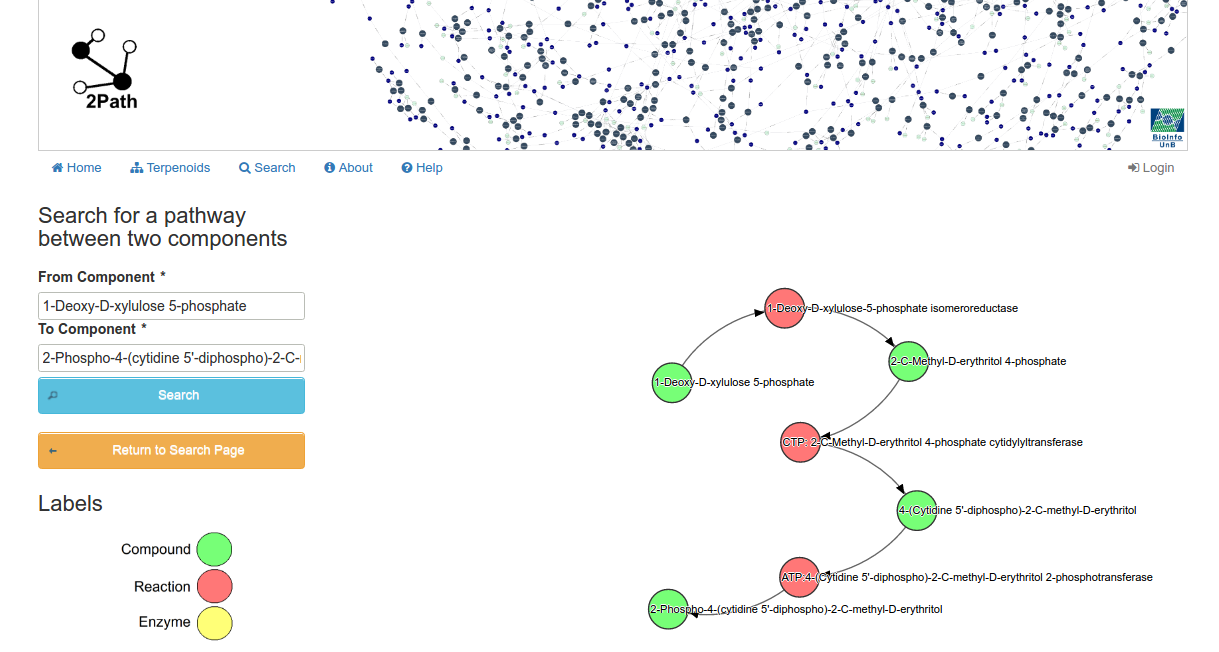
\includegraphics[width=1\textwidth]{new_pathway.png}
    \caption{Resultado de busca por via metabólica em um organismo, onde o grafo gerado possui apenas informação sobre os compostos pesquisados e as reações entre eles.}
    \label{fig:new_pathway}
\end{figure}





  \chapter{Conclusão e Trabalhos Futuros}

\section*{Conclusão}

\indent O \textit{2path} é uma base de conhecimento que preserva as principais características de biossíntese dos terpenos. Ele é capaz de processar um arquivo FASTA e retornar ao usuário um banco modificado, com informações sobre as sequências que geram certas enzimas do banco de dados. Assim, ao pesquisar por uma enzima ou via metabólica em um organismo, o usuário poderia obter todos esses dados. Muitas dessas informações, porém, ou não interessam aos biólogos, ou não devem aparecer em uma visualização interativa com a mesma importância que o que foi buscado de fato.

\indent Nesse sentido, a partir dos testes feitos pelo Método de Avaliação de Comunicabilidade de Interação Humano-Computador, observou-se que a simplicidade do objeto com que o usuário irá interagir é muito mais apreciado do que a quantidade de informação que ele pode obter. Uma interface com poucas páginas e textos é mais simples e, portanto, mais agradável. Uma página com mais informações é mais preferível que uma interface que demanda várias navegações e atualizações de telas.

\section*{Trabalhos Futuros}

\indent A partir da análise dos testes percebeu-se mudanças que poderiam ocorrer no banco de dados 2Path para aumentar a usabilidade de proposta de interface desenvolvida nesse projeto. Essa mudança seria no nó que representam as reações, e a sugestão é de incluir uma propriedade que indica a(s) enzima(s) que às cataliza(m). Com essa informação é possível representar facilmente no grafo as reações com as label do número EC das enzimas que às catalizam. Essa representação do grafo foi solicitado pela maioria dos usuário, que preferem imaginar uma reação como uma aresta do que como um nó, pois quem realiza as reações de fato são as enzimas.
  \appendix

\chapter{Questionários de dados pessoais dos biólogos}\label{questionario_dados_pessoais}

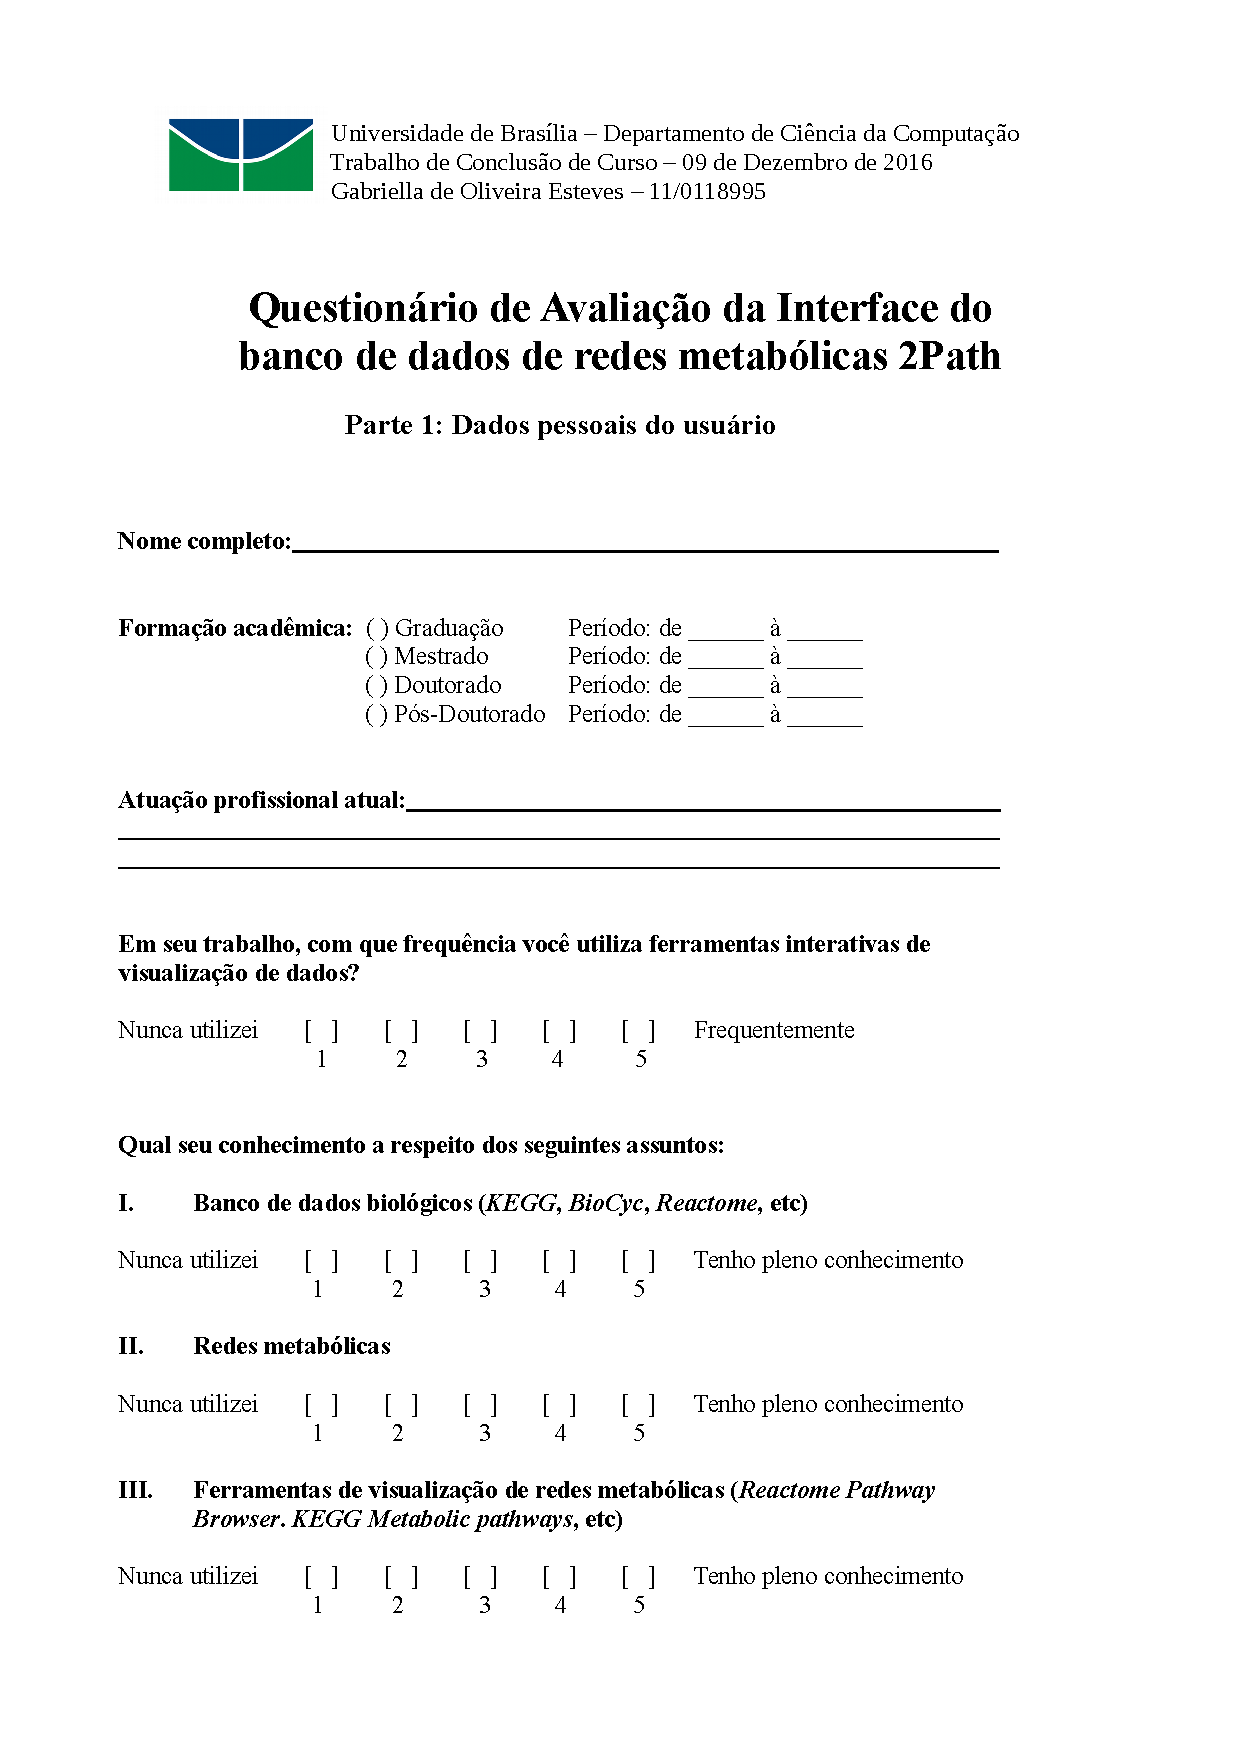
\includepdf[pages={1},scale=1]{capitulos/questionario_dados_pessoais.pdf}

\chapter{Tarefas realizadas pelos biólogos no sistema 2Path}\label{tarefas}

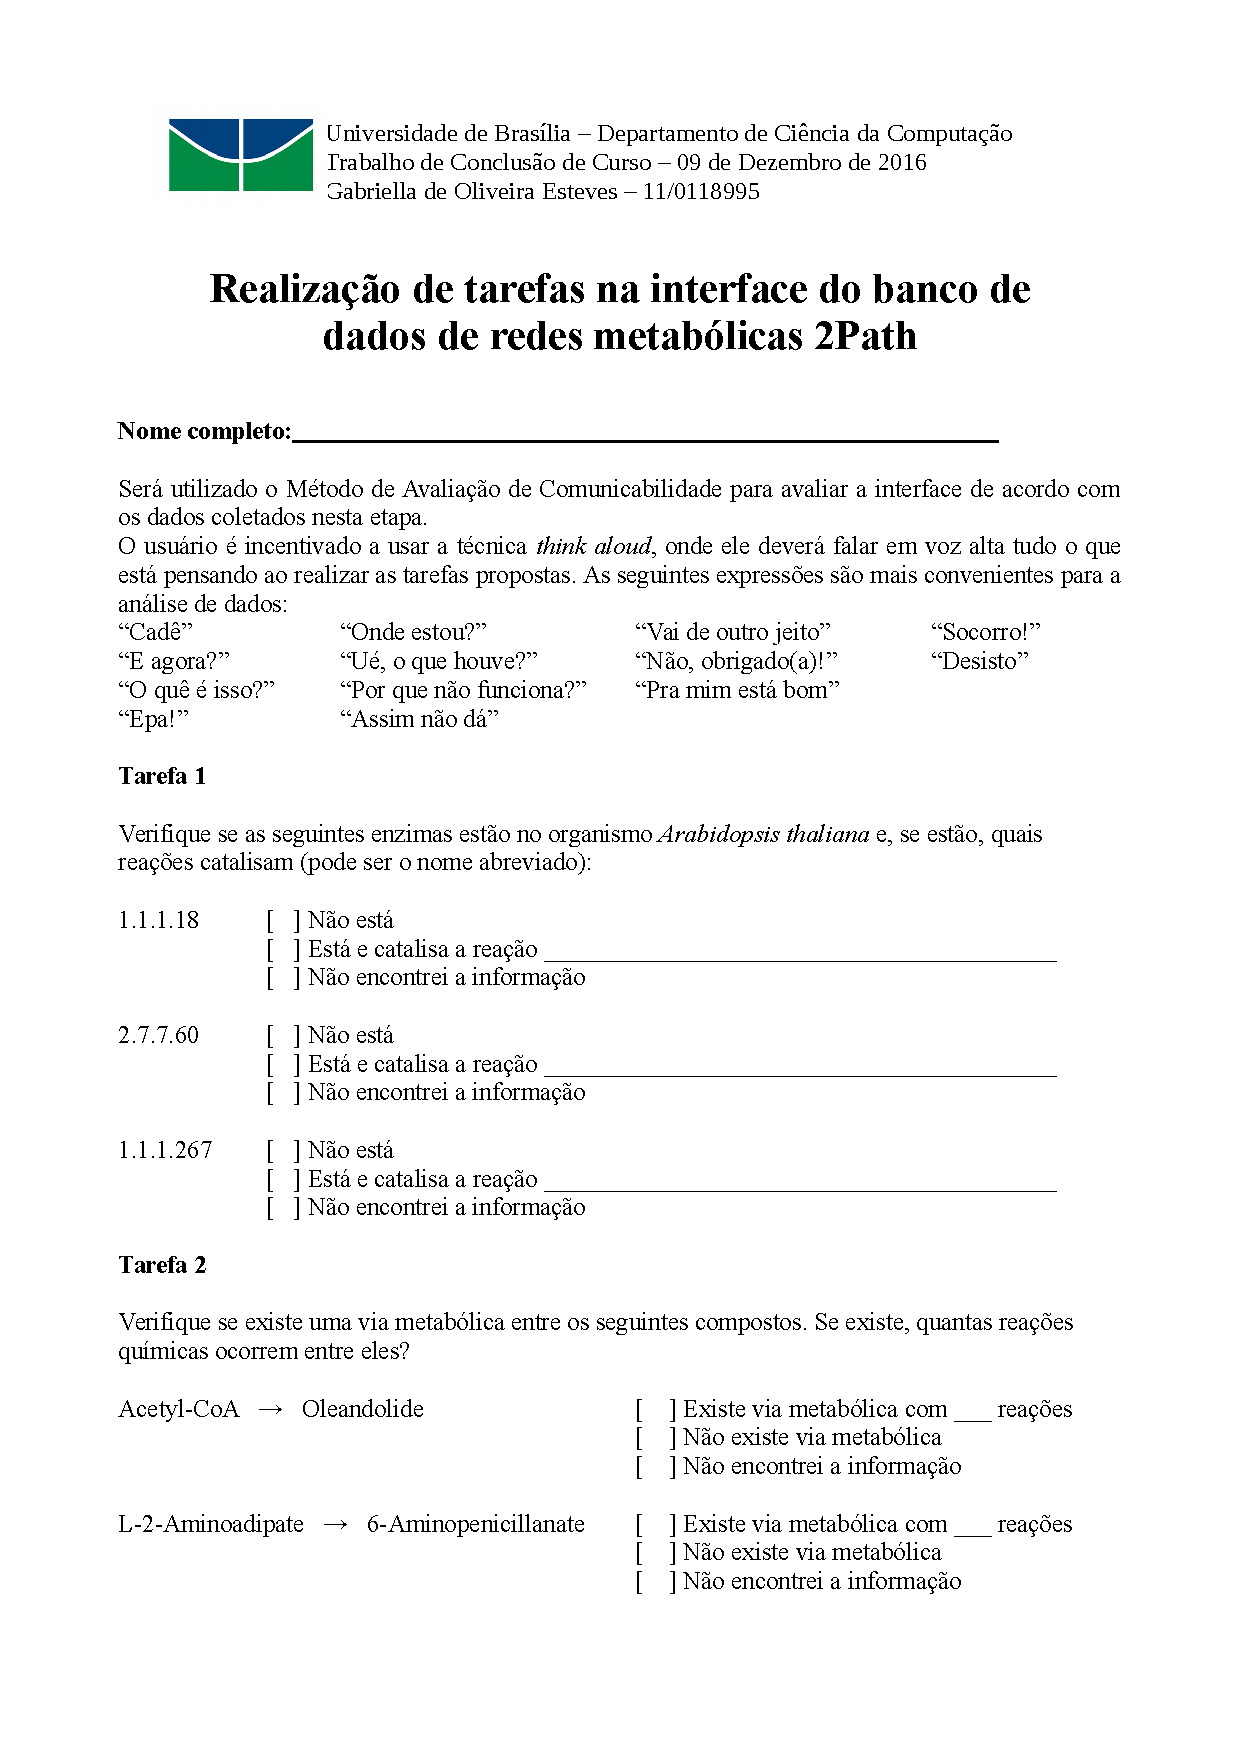
\includepdf[pages={1},scale=1]{capitulos/tarefas_2Path.pdf}

\chapter{Questionários de interface conforme o Método de Avaliação de Comunicabilidade}\label{questionario_interface}

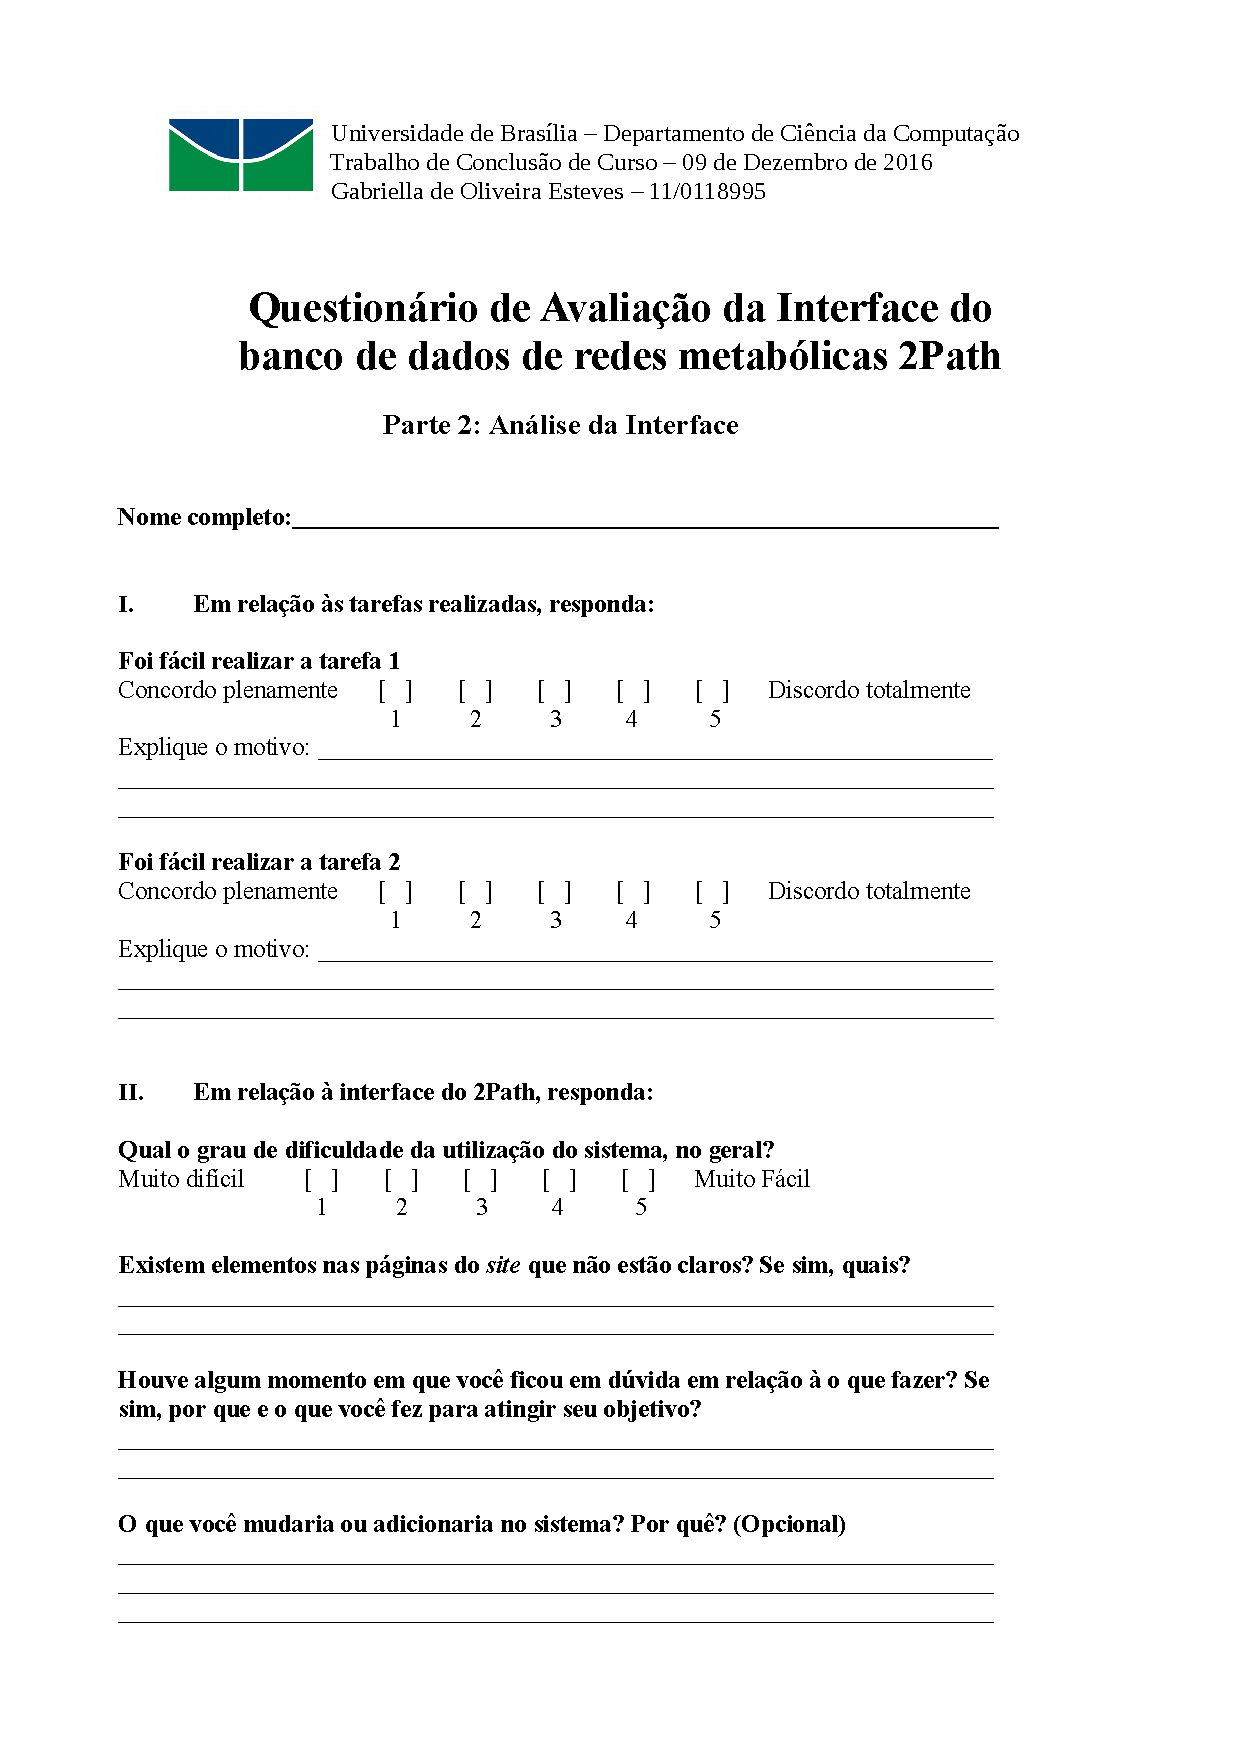
\includepdf[pages={1},scale=1]{capitulos/questionario_interface.pdf}


  \postextual
  \bibliographystyle{plain}
  \bibliography{monografia}

\end{document}
\grid
\grid
